\section{実験}

前節で説明した方法により,15種類のNタプルネットワークのそれぞれについて,Optimistic initialization の初期値 $\mathit{OI}$ を3通り変えて学習を行った.
ランダム性の影響を抑えるため,各条件について乱数のシードを変えて10回の学習を行い,10個のNタプルネットワークを得た.
次に,各Nタプルネットワークに対し,GreedyプレイおよびExpectimax探索(深さ2〜6)により1000ゲームのプレイを行い,それらの平均スコアを求めた.
本節のグラフにおいて,10個のNタプルネットワークの平均を点や線で示し,それらの標準偏差をエラーバー等で示す.

% 本研究では,ミニ2048におけるNタプルネットワークの学習性能を多角的に分析するため,
% 構造の異なる複数のプレイヤを構築し,GreedyおよびExpectimax探索による評価を行った.

% \ref{tuples}で示した15種類のプレイヤを用いて評価を行った.

% さらに,Optimistic Initialization(OI)の影響を調べるため,
% 各プレイヤについてOIの初期値を0,1200,5400に設定し,それぞれ学習を実施した.
% すべてのプレイヤは $5 \times 10^8$ 手分の行動に基づいて学習を行い,
% 乱数シードを変えて10体ずつ学習させた.結果として,
% $15$タプル構成$\times 3$回(OIの初期値)$\times 10$回(シード)で,計$450$体のプレイヤが作成された.

% これらのプレイヤに対して,1000ゲームプレイを行い,
% seed違いの結果をまとめた10000ゲームのログを用いて解析を行なった.

\begin{figure}[t]
    \centering
    \begin{subfigure}[b]{\linewidth}
        \centering
        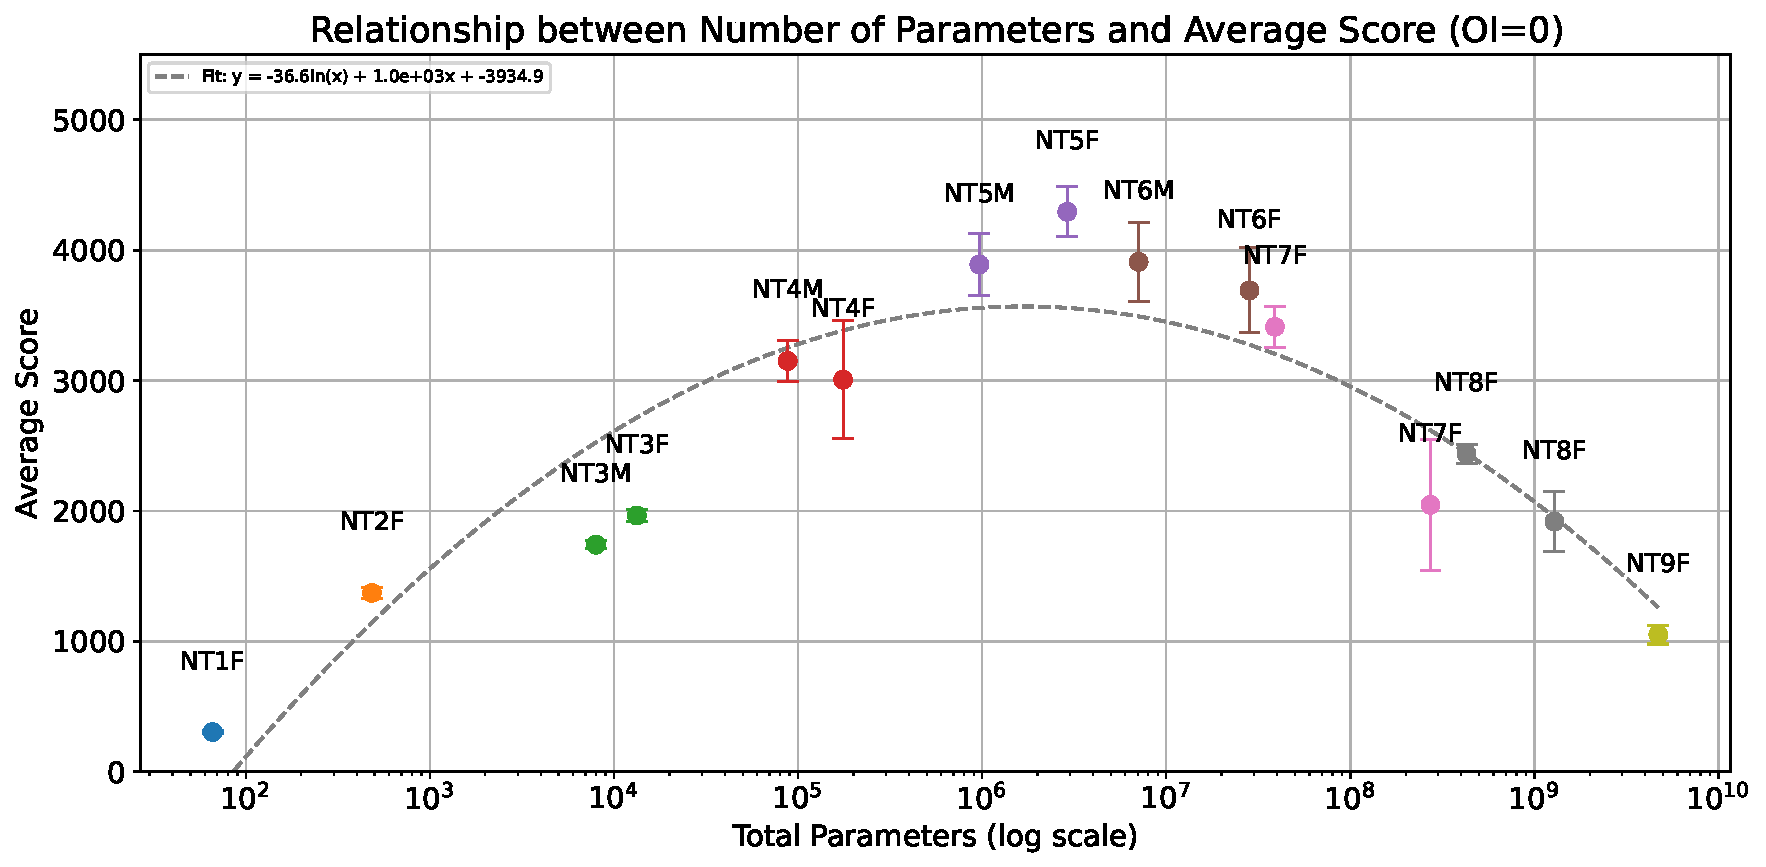
\includegraphics[width=\linewidth]{pdf/parameter_performance_plots/params_performance_OI0_EXP1.pdf}
        \caption{OI=0}
        \label{fig:score_vs_tuple_OI0}
    \end{subfigure}

    \vspace{1em}
    \begin{subfigure}[b]{\linewidth}
        \centering
        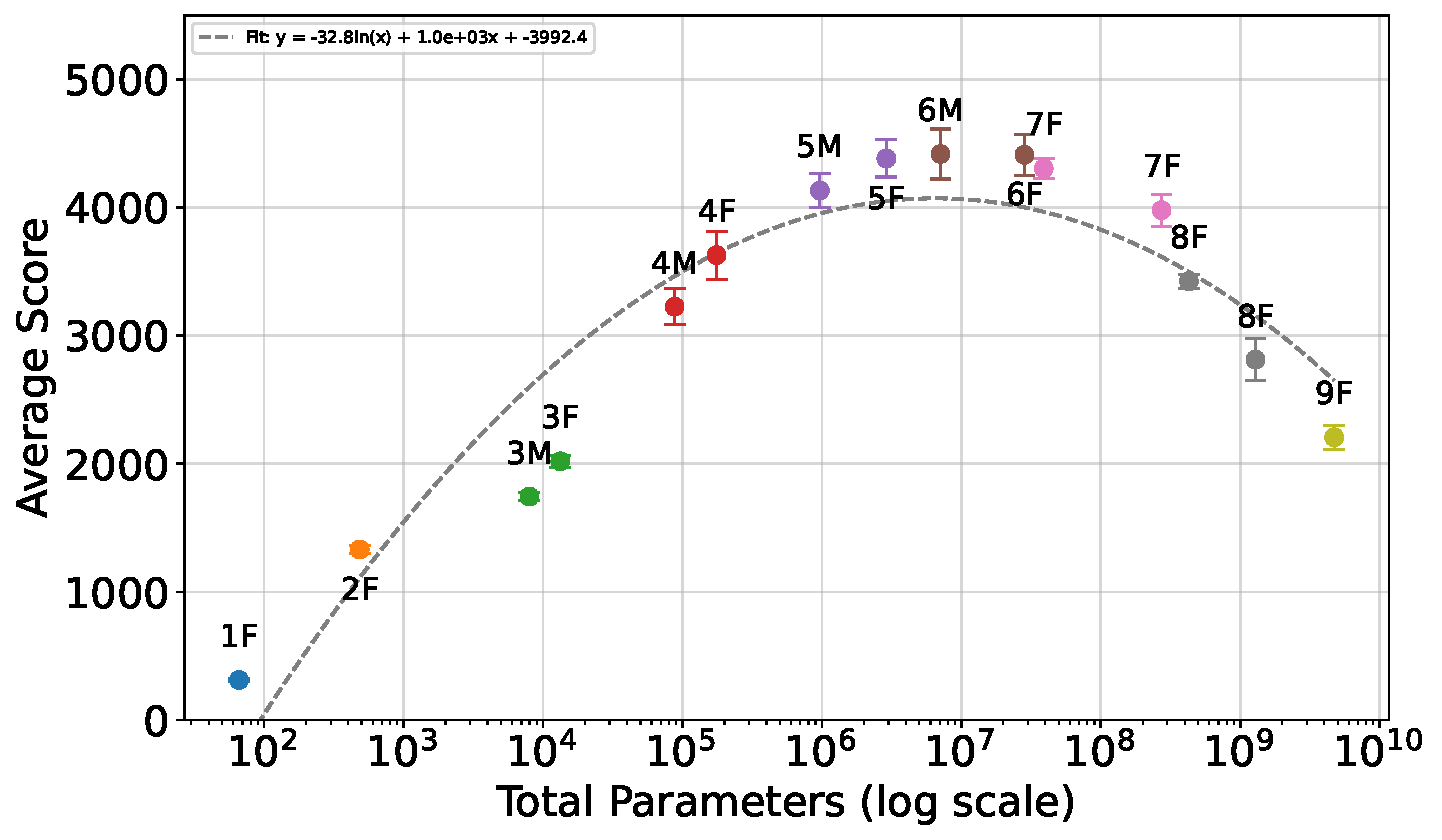
\includegraphics[width=\linewidth]{pdf/parameter_performance_plots/params_performance_OI1200_EXP1.pdf}
        \caption{OI=1200}
        \label{fig:score_vs_tuple_OI1200}
    \end{subfigure}

    \vspace{1em}
    \begin{subfigure}[b]{\linewidth}
        \centering
        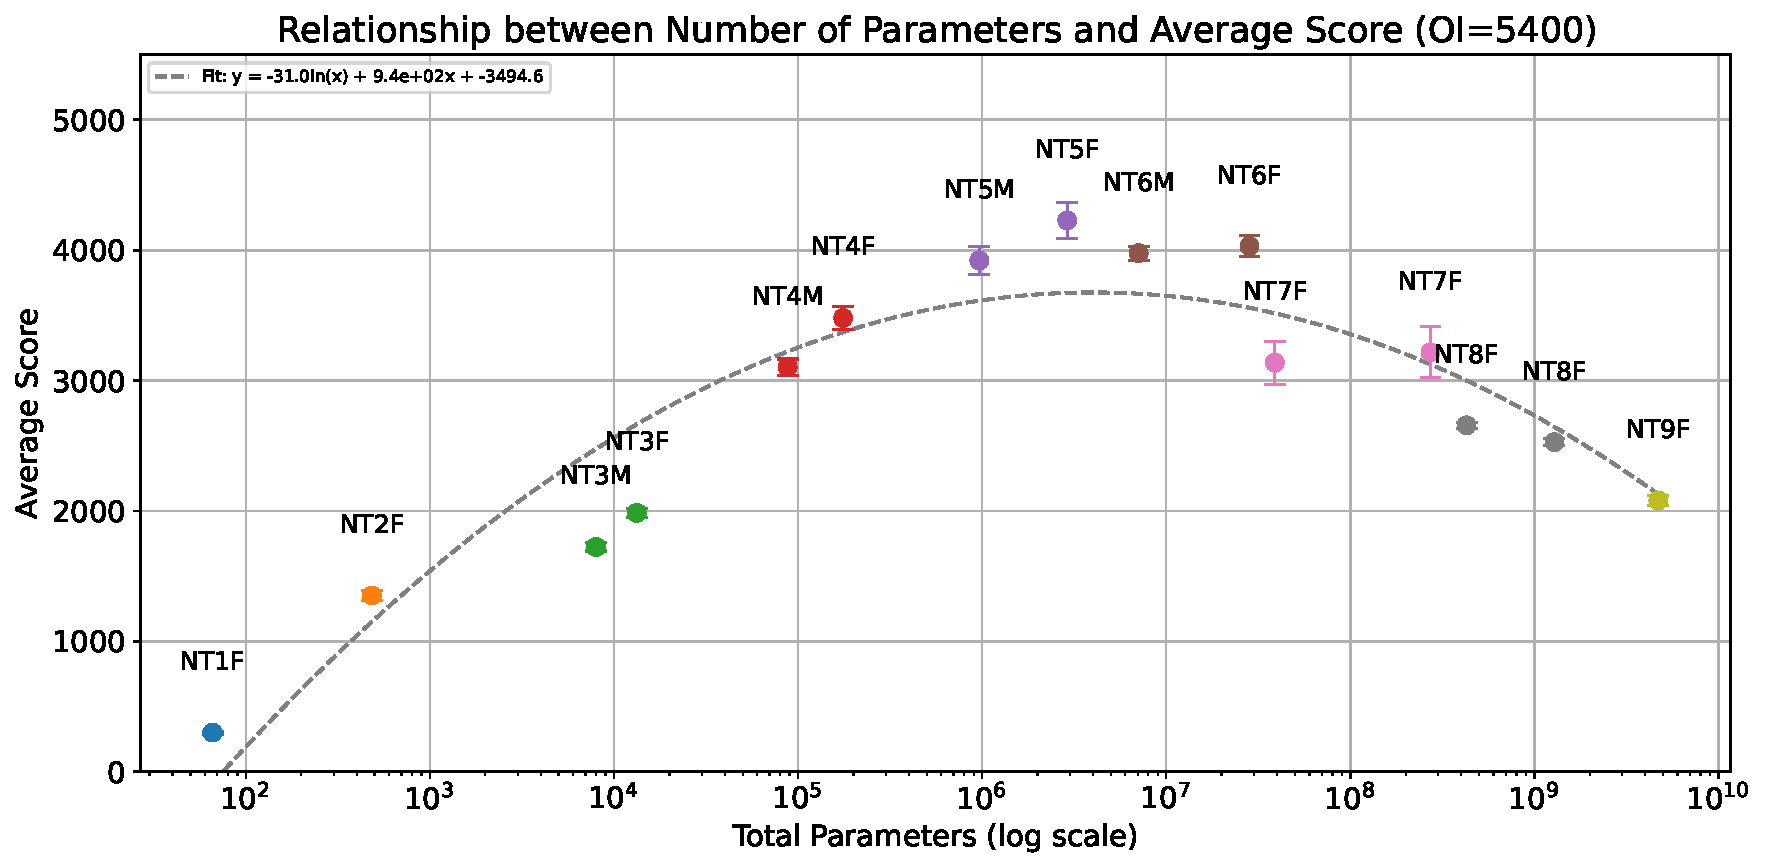
\includegraphics[width=\linewidth]{pdf/parameter_performance_plots/params_performance_OI5400_EXP1.pdf}
        \caption{OI=5400}
        \label{fig:score_vs_tuple_OI5400}
    \end{subfigure}

    \caption{Greedyプレイにおいて,パラメータ数と平均スコアの関係}
    \label{fig:score_vs_tuple_all}
\end{figure}

\begin{figure}[t]
    \centering
    \begin{subfigure}[b]{\linewidth}
        \centering
        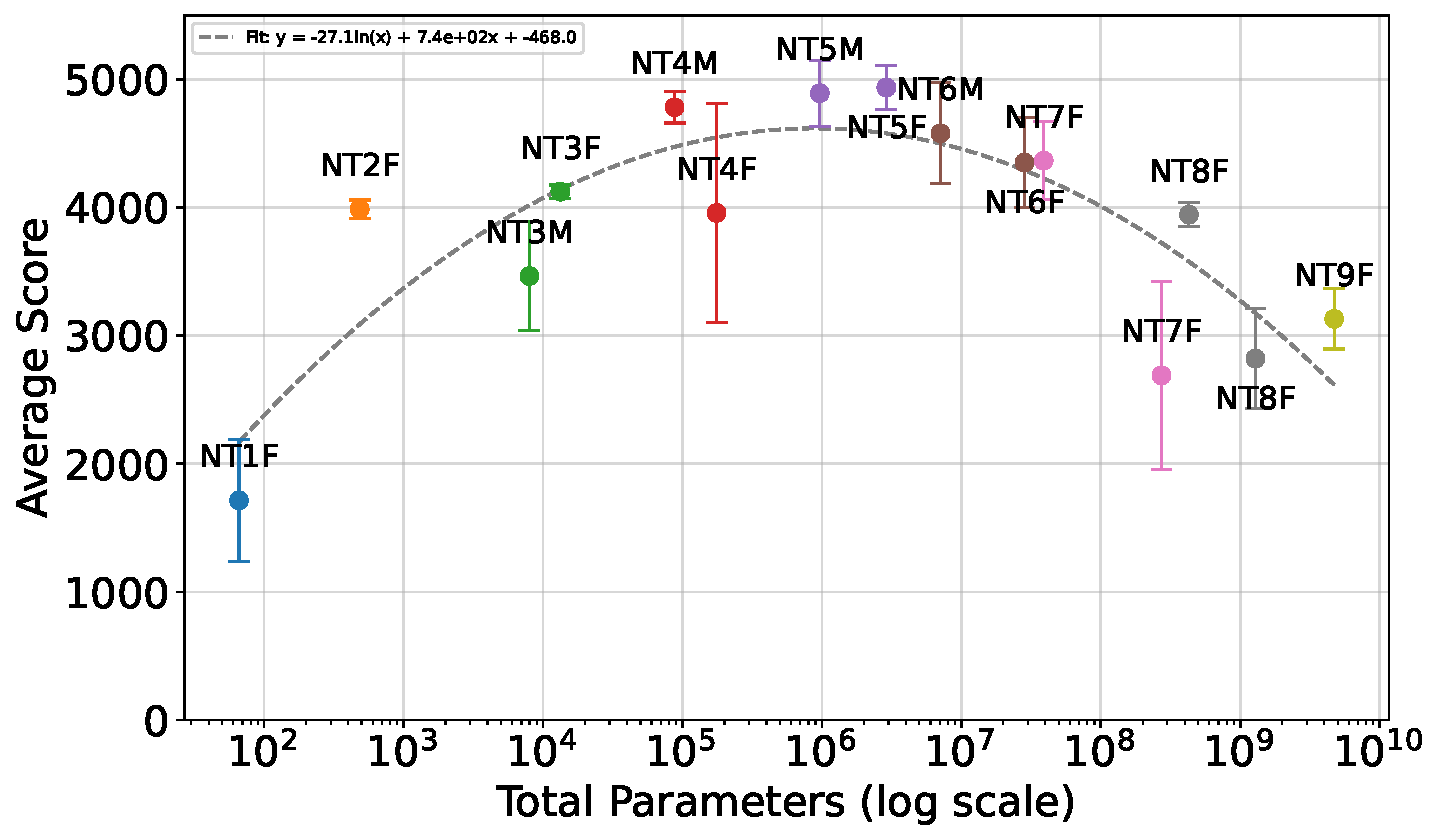
\includegraphics[width=\linewidth]{pdf/parameter_performance_plots/params_performance_OI0_EXP6.pdf}
        \caption{OI=0}
        \label{fig:score_vs_tuple_OI0_EXP6}
    \end{subfigure}

    \vspace{1em}
    \begin{subfigure}[b]{\linewidth}
        \centering
        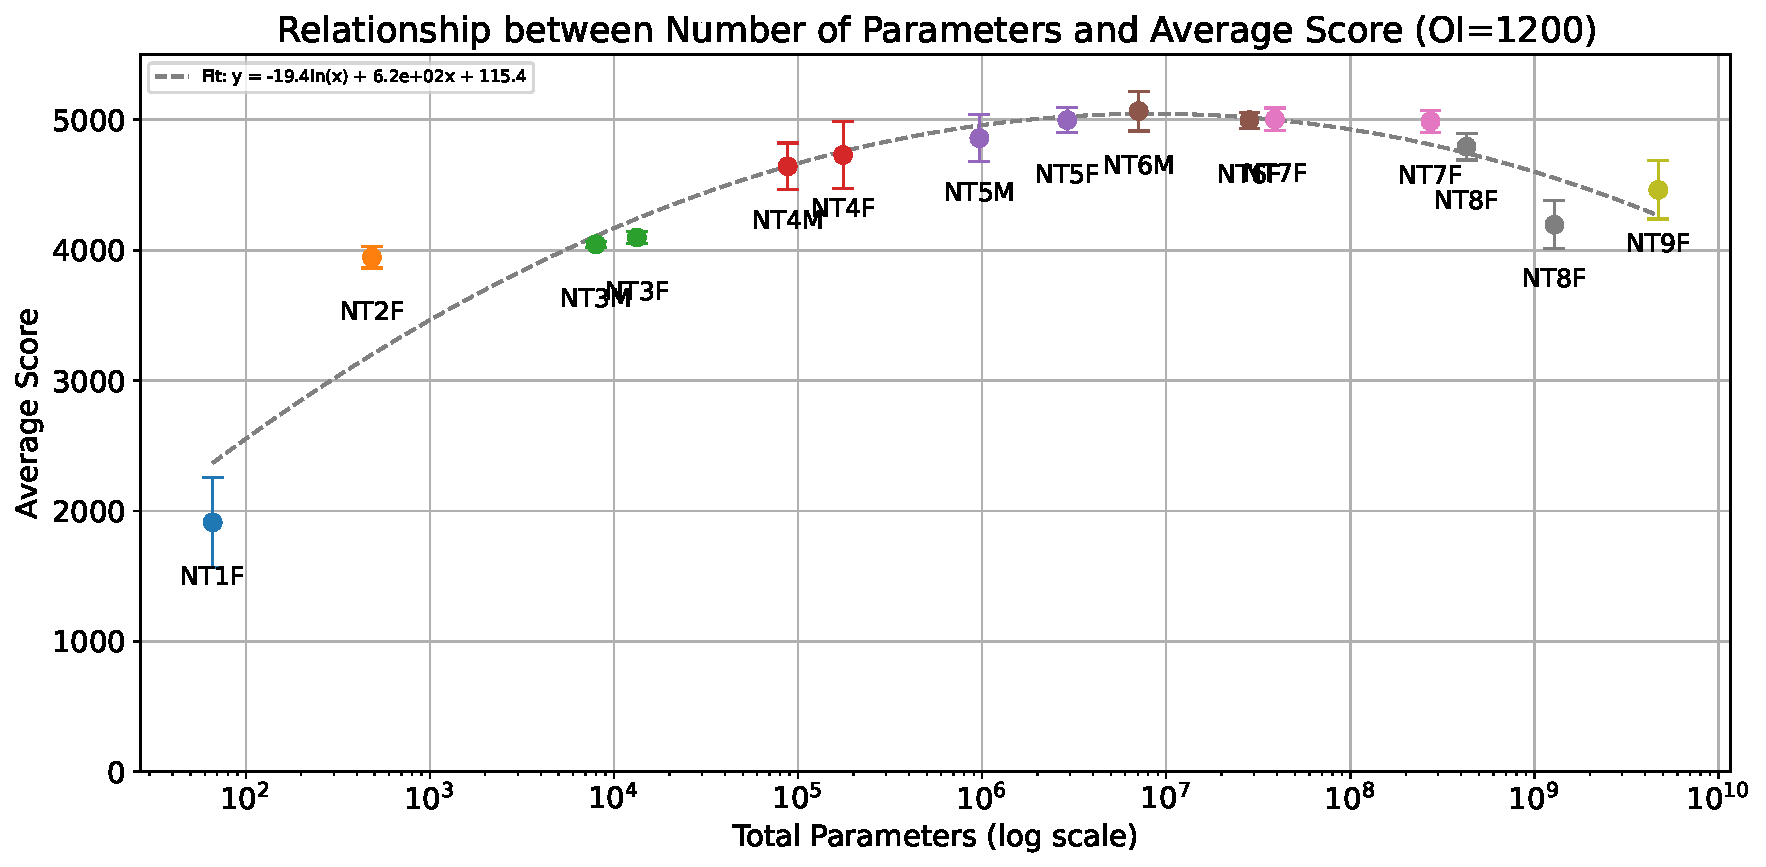
\includegraphics[width=\linewidth]{pdf/parameter_performance_plots/params_performance_OI1200_EXP6.pdf}
        \caption{OI=1200}
        \label{fig:score_vs_tuple_OI1200_EXP6}
    \end{subfigure}

    \vspace{1em}
    \begin{subfigure}[b]{\linewidth}
        \centering
        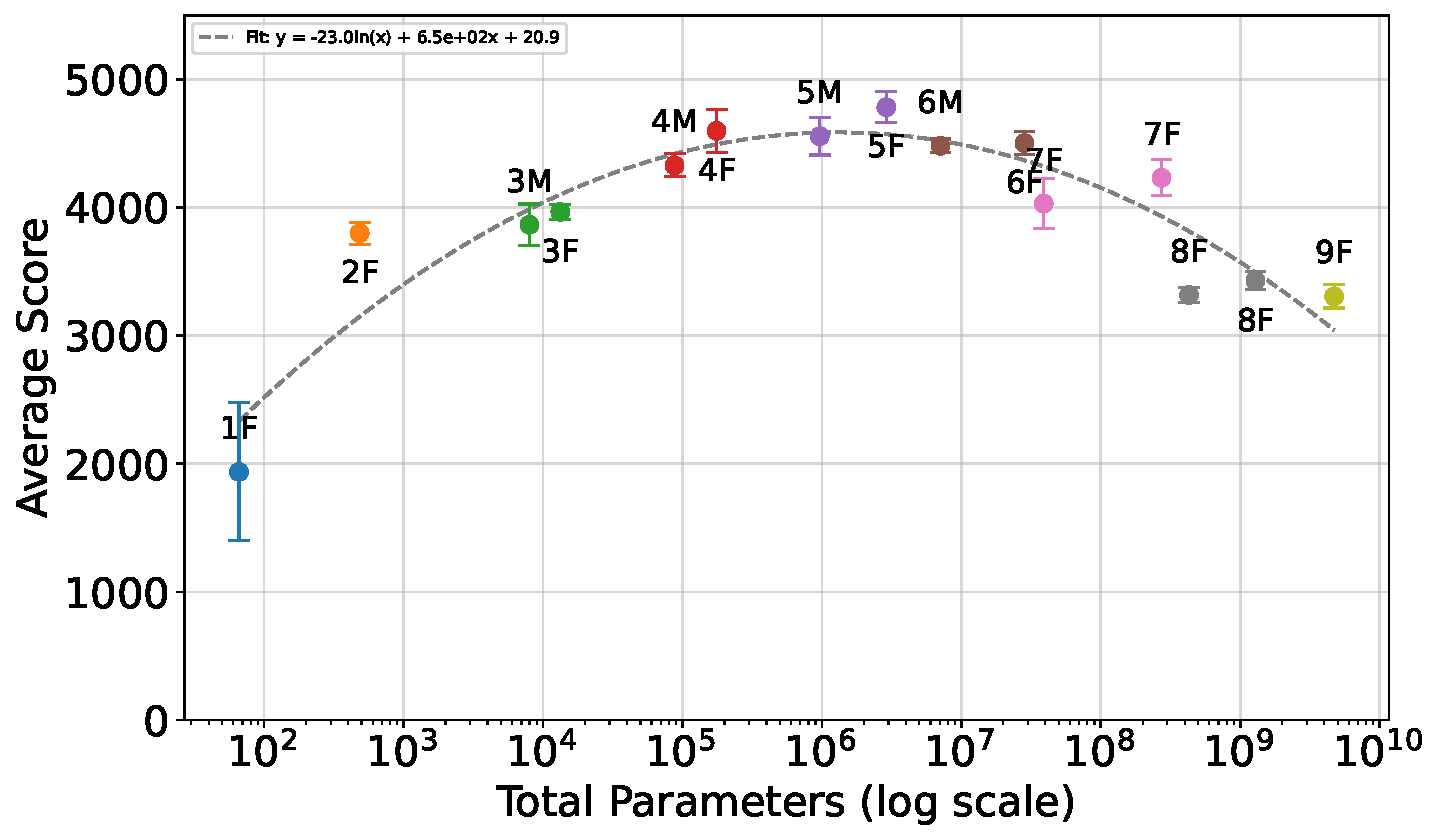
\includegraphics[width=\linewidth]{pdf/parameter_performance_plots/params_performance_OI5400_EXP6.pdf}
        \caption{OI=5400}
        \label{fig:score_vs_tuple_OI5400_EXP6}
    \end{subfigure}

    \caption{Expectimax深さ6において,パラメータ数と平均スコアの関係}
    \label{fig:score_vs_tuple_all_EXP6}
\end{figure}

\subsection{スコアとパラメータ数の関係}
第1節で示した RQ1 について考察するため,Greedy プレイのスコアを,Optimistic initialization の初期値($\mathit{OI}$)ごとにプロットしたものが図\ref{fig:score_vs_tuple_OI0}から図\ref{fig:score_vs_tuple_OI5400}である.これらのグラフは,横軸にパラメータ数の対数をとり,縦軸にスコアの平均値と標準偏差をプロットしている.また,それぞれのグラフの点に対し,パラメータ数の対数とスコアの関係を二次関数でフィッティングして得られる近似曲線も描いている.

これらのグラフから,いずれのグラフもおよそ放物線を描いていることが分かる.
とくに,\textsf{5M}から\textsf{6F}の区間に放物線の頂点が位置することが確認できた.
また,$\mathit{OI}=0$の場合(図\ref{fig:score_vs_tuple_OI0}),3種類の初期値の中で標準偏差が大きいものが目立っている.このことは,Optimistic initializationを行わない学習では,学習の幅広さが足りず,安定的に良い結果が得られないことを意味する.
$\mathit{OI}=1200$ と $\mathit{OI}=5400$の場合(図\ref{fig:score_vs_tuple_OI1200},図\ref{fig:score_vs_tuple_OI5400}),スコアのばらつきは小さい.
また,より多くのパラメータ数のところまでスコアの向上が見られる(すなわち,放物線の頂点が右に移動する).
\textsf{5F}よりもパラメータ数の少ないNタプルネットワークでは,平均スコアは初期値にそれほど依存していない.一方,それよりも多くのパラメータを持つNタプルネットワークでは,初期値が $\mathit{OI}=1200$ の場合に最も良い結果が得られた.

次に,RQ1 と RQ3 について考察するため,深さ6のExpectimax探索を行った場合の,Nタプルネットワークのパラメータ数と平均スコアを関係を図\ref{fig:score_vs_tuple_OI0_EXP6}から図\ref{fig:score_vs_tuple_OI5400_EXP6}に示す.
各グラフの近似曲線から,いずれのグラフもおよそ放物線を描いていること,いずれの平均スコアもGreedyプレイのスコアよりも高いことが確認できた.

$\mathit{OI}=0$ の場合,探索を行ってもスコアのばらつきはそれほど小さくならず,特に Full のものについてばらつきが大きい傾向が見られる.
これはパラメータ数が多い方が評価値の修正が起こり難く,局所最適解から抜け出しにくいのではないかと考えられる.

$\mathit{OI}=1200$ の場合,\textsf{5M}から\textsf{7F}まで同程度の平均スコアを達成しており,放物線の上昇と下降の傾きが小さい.
これは,強いプレイヤが達成しうるスコアの上限に近づいていて向上の余地が小さいことと,弱いプレイヤが探索によってスコアを上昇させられることを示唆する.
$\mathit{OI}=5400$ の場合には,スコアのばらつきは小さいものの,放物線の形やスコアの最大は $\mathit{OI}=0$ の場合のそれらとあまり変わらなかった.


\subsection{学習の進み方の比較}

RQ2 について考察するため,\textsf{5M}と\textsf{7M}を例にとり,学習過程のスコアの推移を確認した.図\ref{fig:learning_progress_comparison}は,横軸に学習ステップ数を,縦軸にスコアをとり,学習ステップ10000ごとに学習エピソードの平均をプロットしたものである.

Optimistic initializationの初期値を $\mathit{OI}=0$ と設定した場合,\textsf{5M}では学習が進むにつれてスコアが上昇しているが,\textsf{7F}ではスコアが上昇していない.
これは\textsf{7F}が局所最適解にハマっていることを示唆する.

初期値を$\mathit{OI}=1200$と設定した場合,\textsf{5M}と\textsf{7F}の両方でスコアの上昇が $\mathit{OI}=0$ の場合よりも緩やかになった.
詳しく見ると,\textsf{5M}では,約2800点を達成したあたりで途中一度停滞しており,その後再びスコアの上昇に転じている.
表\ref{specific}より,約2800点というのは256タイルが完成してから512タイルが完成するまでの間であることが分かる.
この間の盤面では空きタイルが多くあるため,学習に出現する盤面の種類が多いことが停滞の原因ではないかと考えている.
また,\textsf{7F}において初期値を $\mathit{OI}=1200$ と設定した場合,序盤のスコアの上昇が緩やかになっているが,これも同じ原因ではないかと考える.

初期値を $\mathit{OI}=5400$ と設定した場合,\textsf{5M}と\textsf{7F}の両方でスコアの上昇が緩やかになり,途中で停滞が発生している.
\textsf{5M}では停滞を乗り越えて大きくスコアを上昇させることに成功しているが,\textsf{7F}では停滞が長引いてしまい結果として学習不足であることが判明した.

\begin{figure}[t]
    \centering
    \begin{subfigure}[b]{\linewidth}
        \centering
        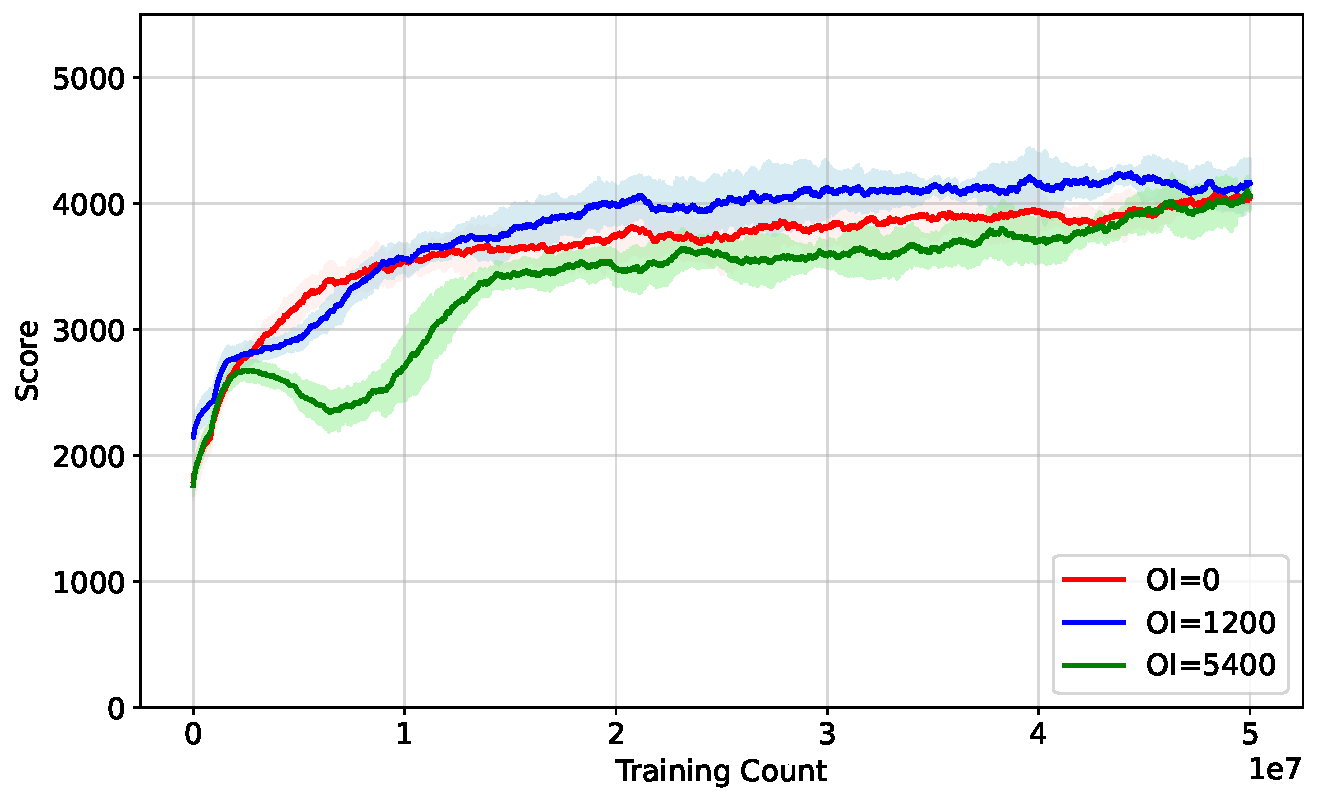
\includegraphics[width=\linewidth]{pdf/learning_progress_plots/learning_progress_NT5M_tuple298_combined.pdf}
        \caption{5Mの学習過程のスコアの変化}
        \label{fig:learning_progress_NT5M}
    \end{subfigure}

    \vspace{1em}
    \begin{subfigure}[b]{\linewidth}
        \centering
        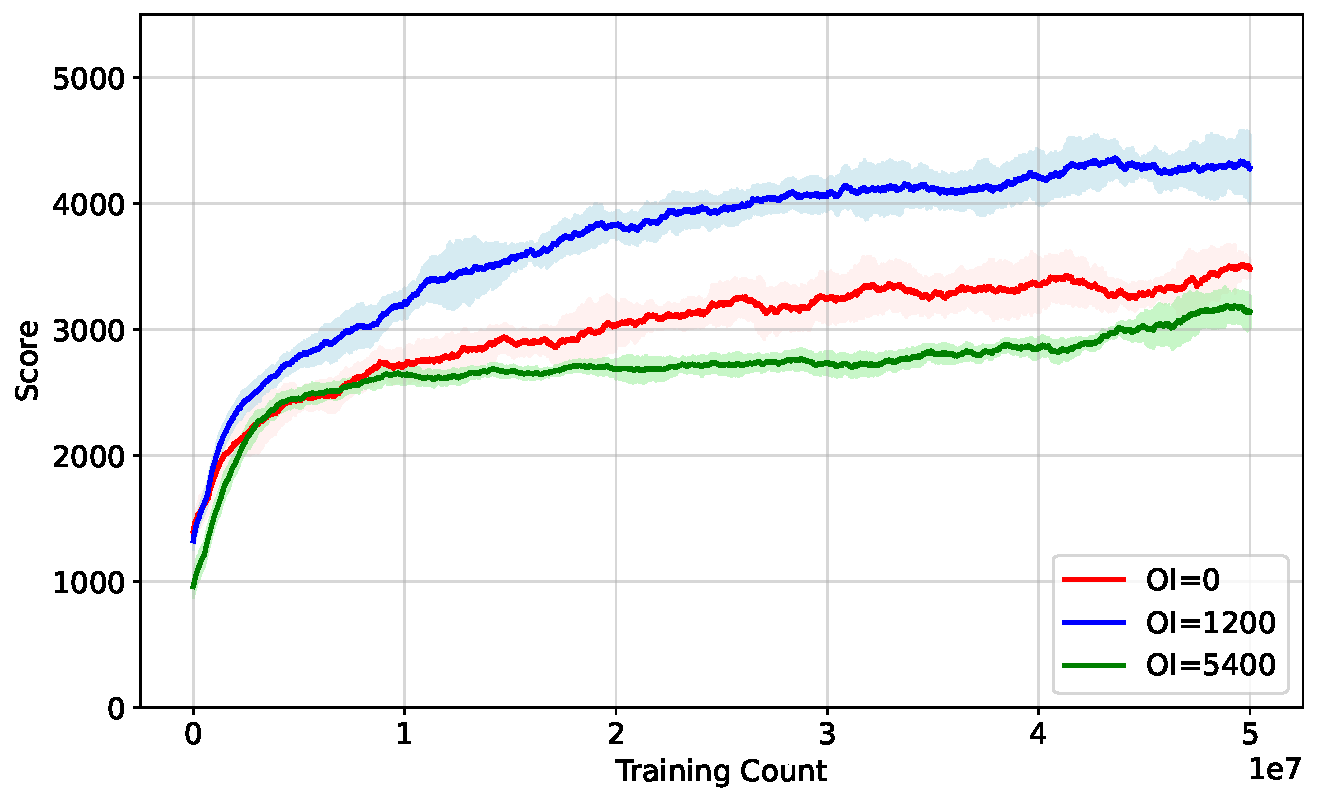
\includegraphics[width=\linewidth]{pdf/learning_progress_plots/learning_progress_NT7F_tuple0_combined.pdf}
        \caption{7Fの学習過程のスコアの変化}
        \label{fig:learning_progress_NT7F}
    \end{subfigure}

    \caption{5Mと7Fの学習推移の比較}
    \label{fig:learning_progress_comparison}
\end{figure}

\subsection{パラメータ数の増加によるプレイヤの挙動の変化}
ここからOIの初期値1200のスコアが同等でパラメータ数が違う4Fと8M,5Mと7Fのプレイヤを比較して,
パラメータ数の増加がプレイヤの挙動にどのような影響を与えるのかについて詳しく調べて行く.
\begin{figure}[t]
\centering
\begin{subfigure}[b]{0.8\linewidth}
    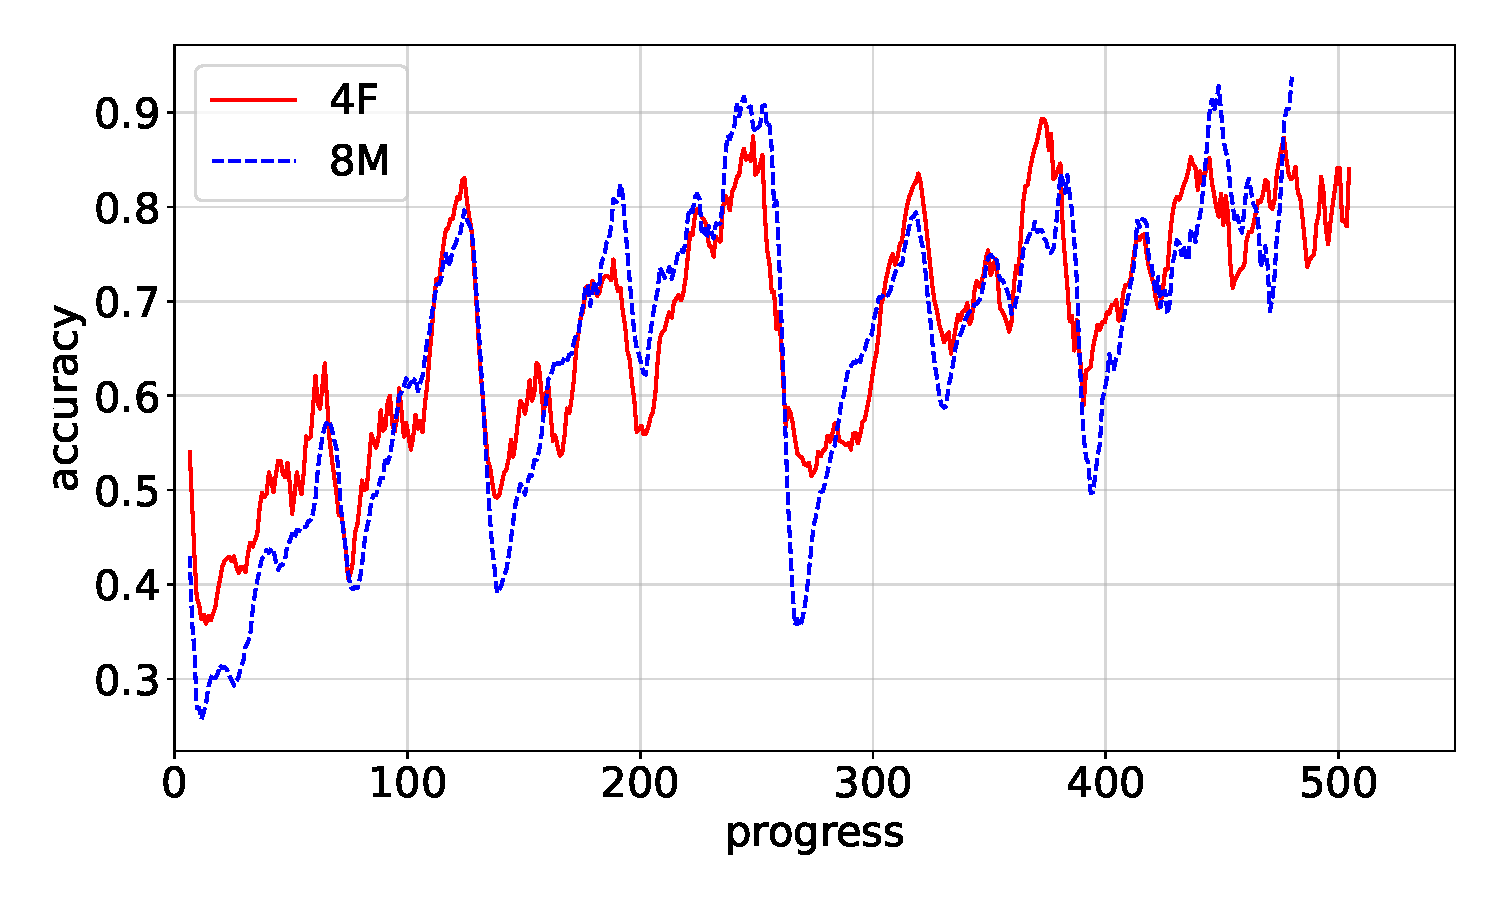
\includegraphics[width=\linewidth]{pdf/compare/NT4F_and_NT8M/accuracy.pdf}
    \caption{正確度}
    \label{fig:NT4F_and_NT8M_accuracy}
\end{subfigure}
% \begin{subfigure}[b]{0.8\linewidth}
%     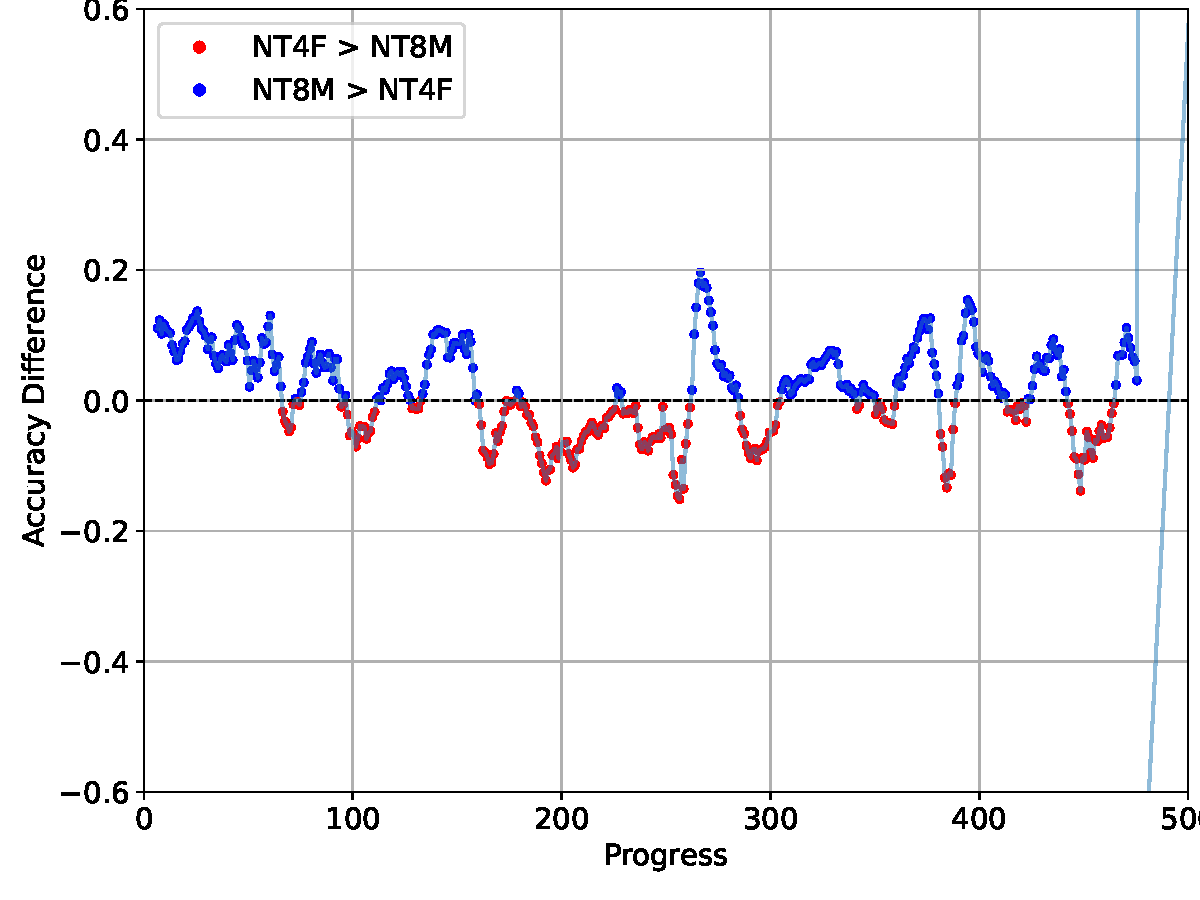
\includegraphics[width=\linewidth]{pdf/compare/NT4F_and_NT8M/acc_diff_plot.pdf}
%     \caption{正確度の差分}
%     \label{fig:NT4F_and_NT8M_acc_diff}
% \end{subfigure}
% \begin{subfigure}[b]{0.49\linewidth}
%     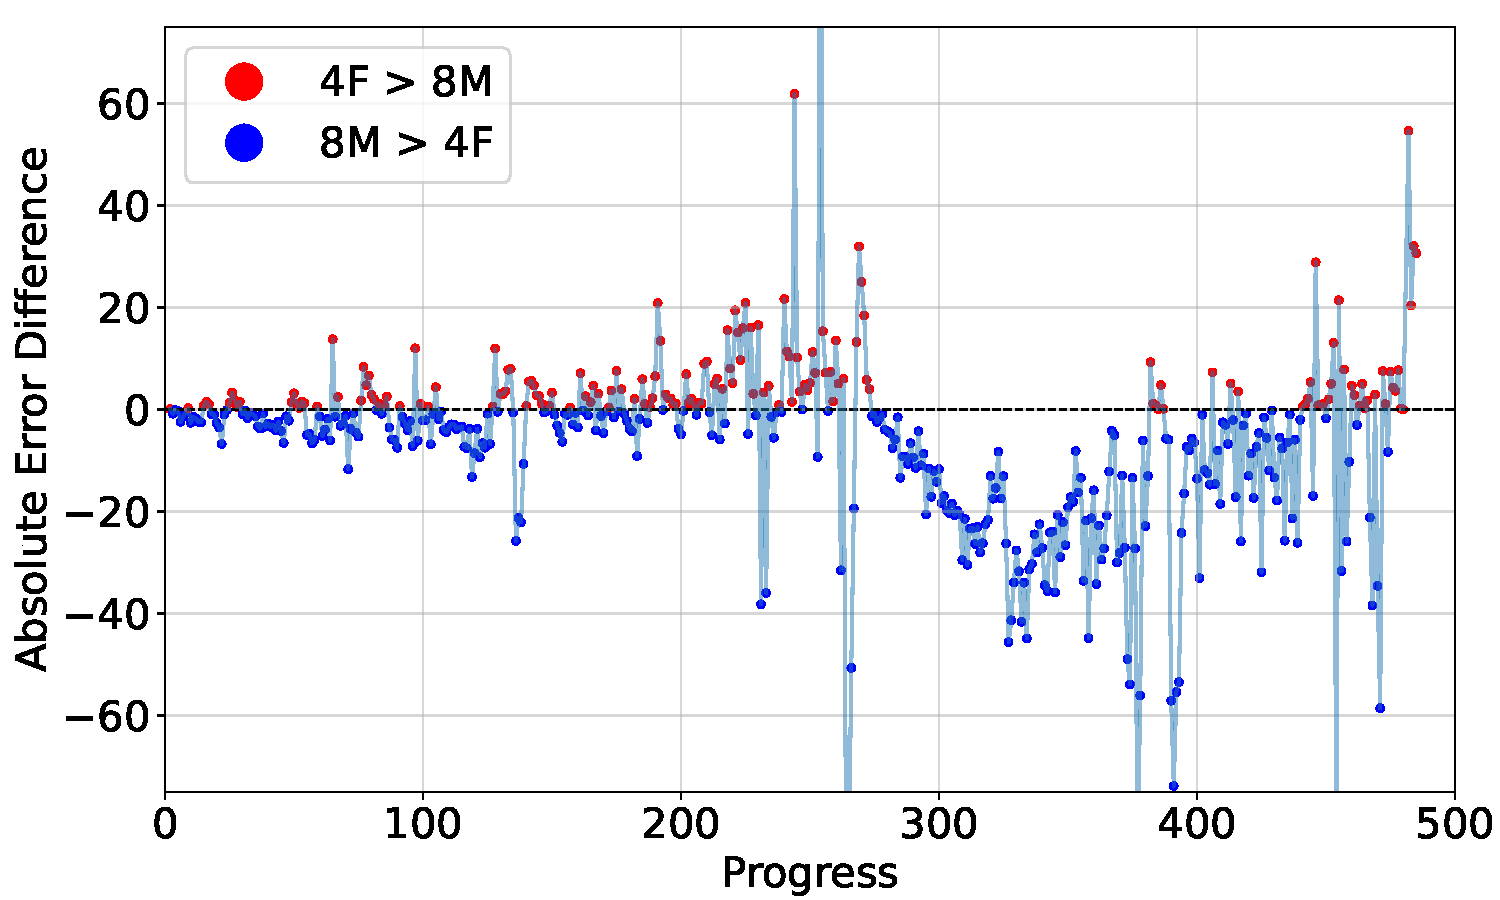
\includegraphics[width=\linewidth]{pdf/compare/NT4F_and_NT8M/error_abs_diff_plot.pdf}
%     \caption{絶対誤差の差分}
%     \label{fig:NT4F_and_NT8M_error_abs_diff}
% \end{subfigure}
\begin{subfigure}[b]{0.8\linewidth}
    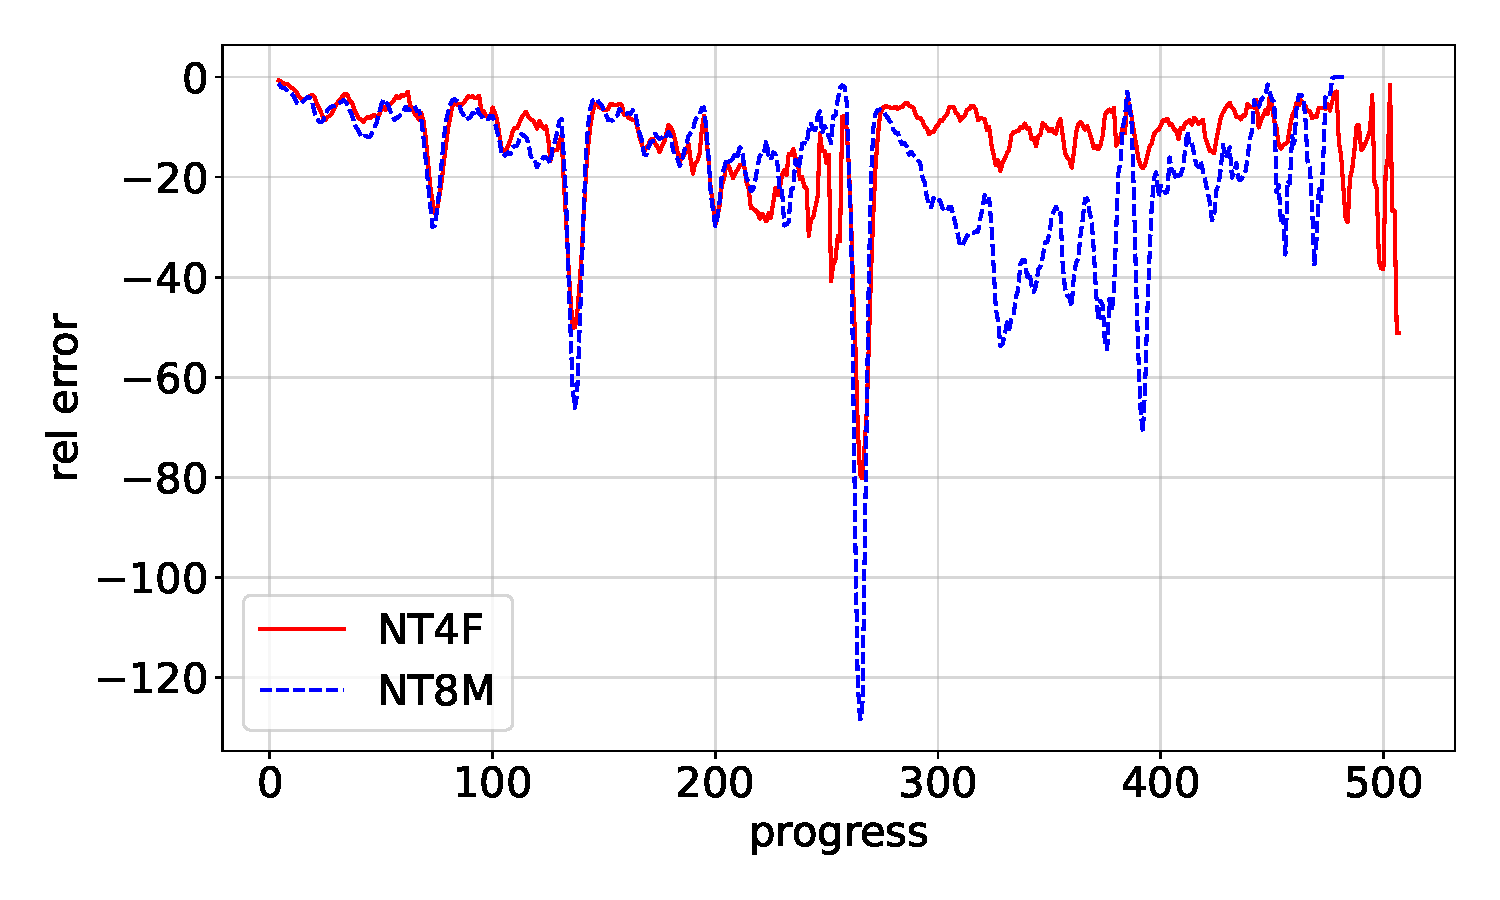
\includegraphics[width=\linewidth]{pdf/compare/NT4F_and_NT8M/error_abs.pdf}
    \caption{絶対誤差}
    \label{fig:NT4F_and_NT8M_error_abs_diff}
\end{subfigure}
\begin{subfigure}[b]{0.8\linewidth}
    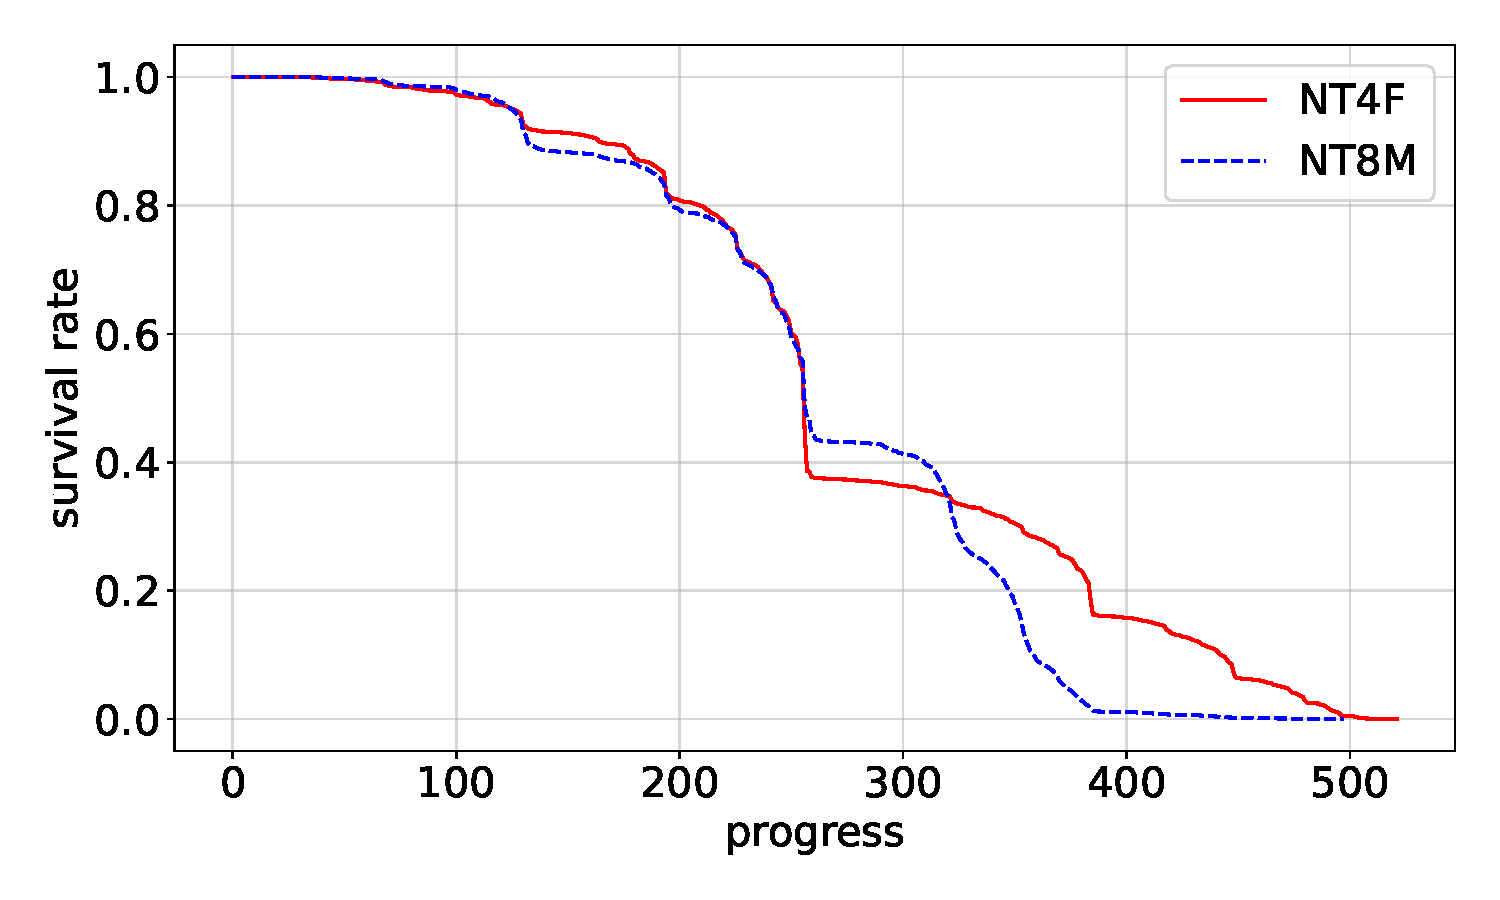
\includegraphics[width=\linewidth]{pdf/compare/NT4F_and_NT8M/survival.pdf}
    \caption{生存率}
    \label{fig:NT4F_and_NT8M_survival}
\end{subfigure}
\caption{4Fと8Mの比較結果}
\label{fig:NT4F_and_NT8M_results}
\end{figure}

まず初めに図\ref{fig:NT4F_and_NT8M_results}は,4Fと8MのプレイヤのGreedyプレイの比較を示している.
\ref{fig:NT4F_and_NT8M_accuracy}と\ref{fig:NT4F_and_NT8M_acc_diff}は,4Fと8Mのプレイヤの正確度を示している.
これを見ると序盤は4Fの方が正確度が高いが,中盤以降はどちらも抜きつ抜かれつの状態であることが分かる.
\ref{fig:NT4F_and_NT8M_error_abs_diff}は,4Fと8Mのプレイヤの絶対誤差の差分を示している.
これを見ると,4Fの方が8M多くのprogressで絶対誤差が小さいことが分かる.
正確度のグラフと絶対誤差のグラフを合わせてみると,4Fの方が後半かなり良いことがわかる.
これは\ref{fig:NT4F_and_NT8M_survival}の生存率のグラフにも表れている.

\begin{figure}[t]
\centering
\begin{subfigure}[b]{0.8\linewidth}
    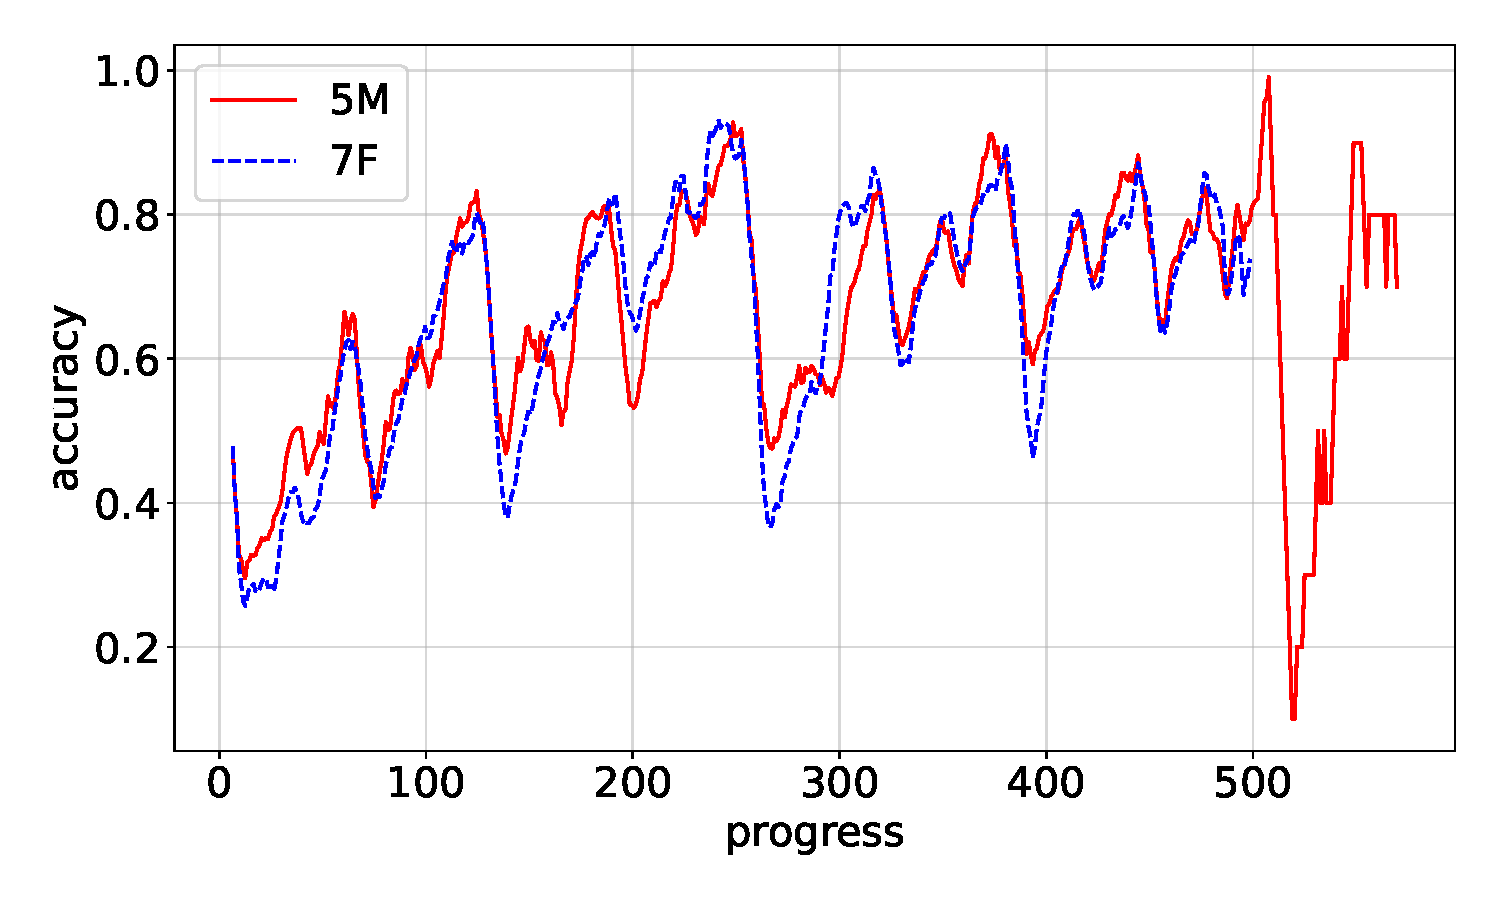
\includegraphics[width=\linewidth]{pdf/compare/NT5M_and_NT7F/accuracy.pdf}
    \caption{正確度}
    \label{fig:NT5M_and_NT7F_accuracy}
\end{subfigure}
% \begin{subfigure}[b]{0.8\linewidth}
%     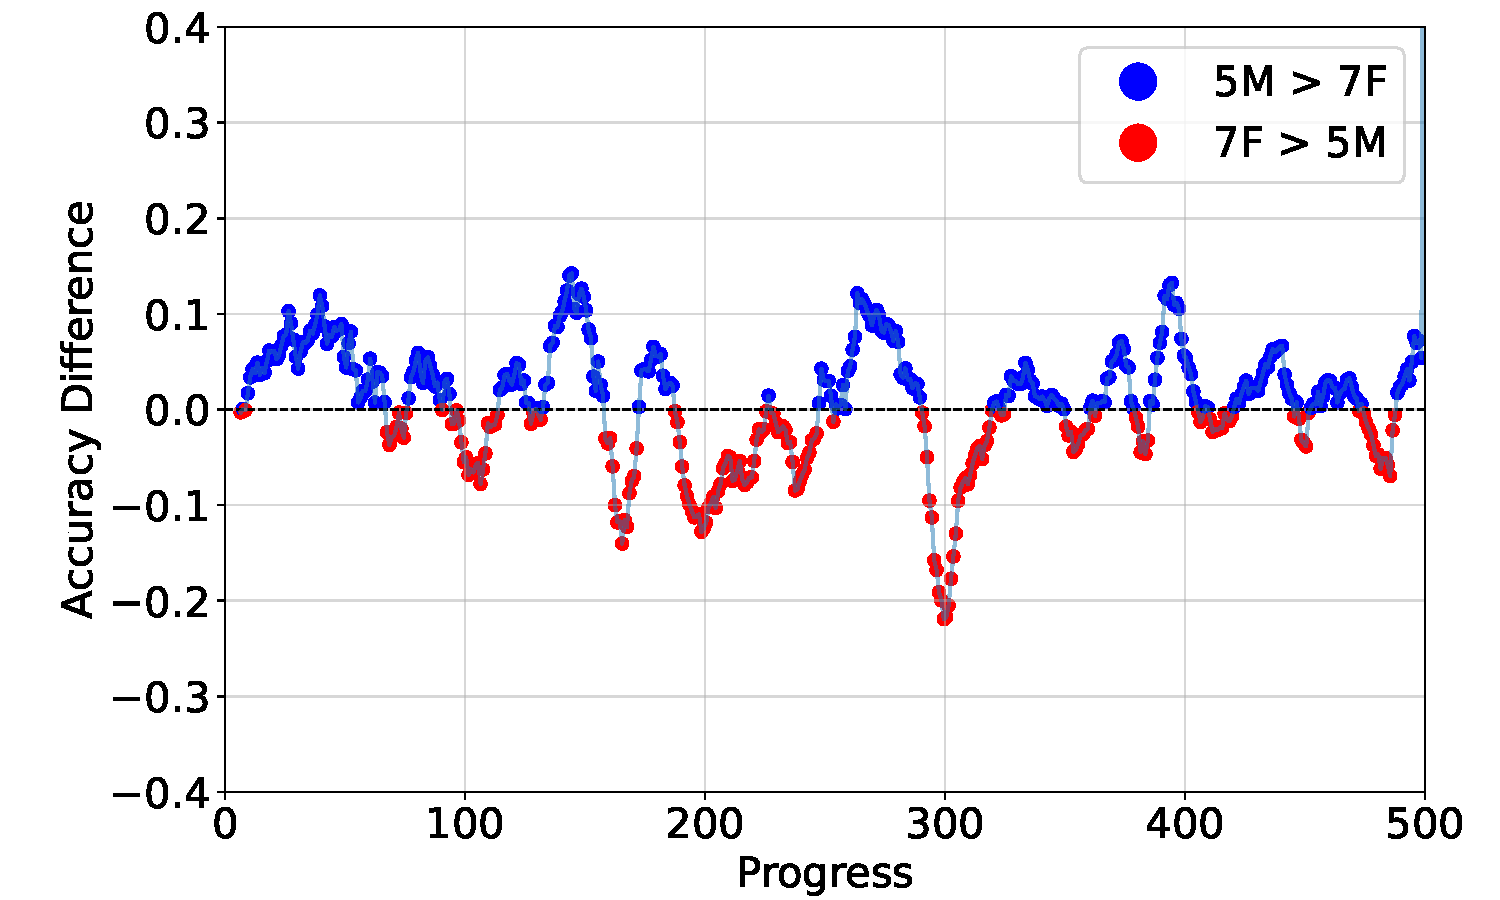
\includegraphics[width=\linewidth]{pdf/compare/NT5M_and_NT7F/acc_diff_plot.pdf}
%     \caption{正確度の差分}
%     \label{fig:NT5M_and_NT7F_acc_diff}
% \end{subfigure}
\begin{subfigure}[b]{0.8\linewidth}
    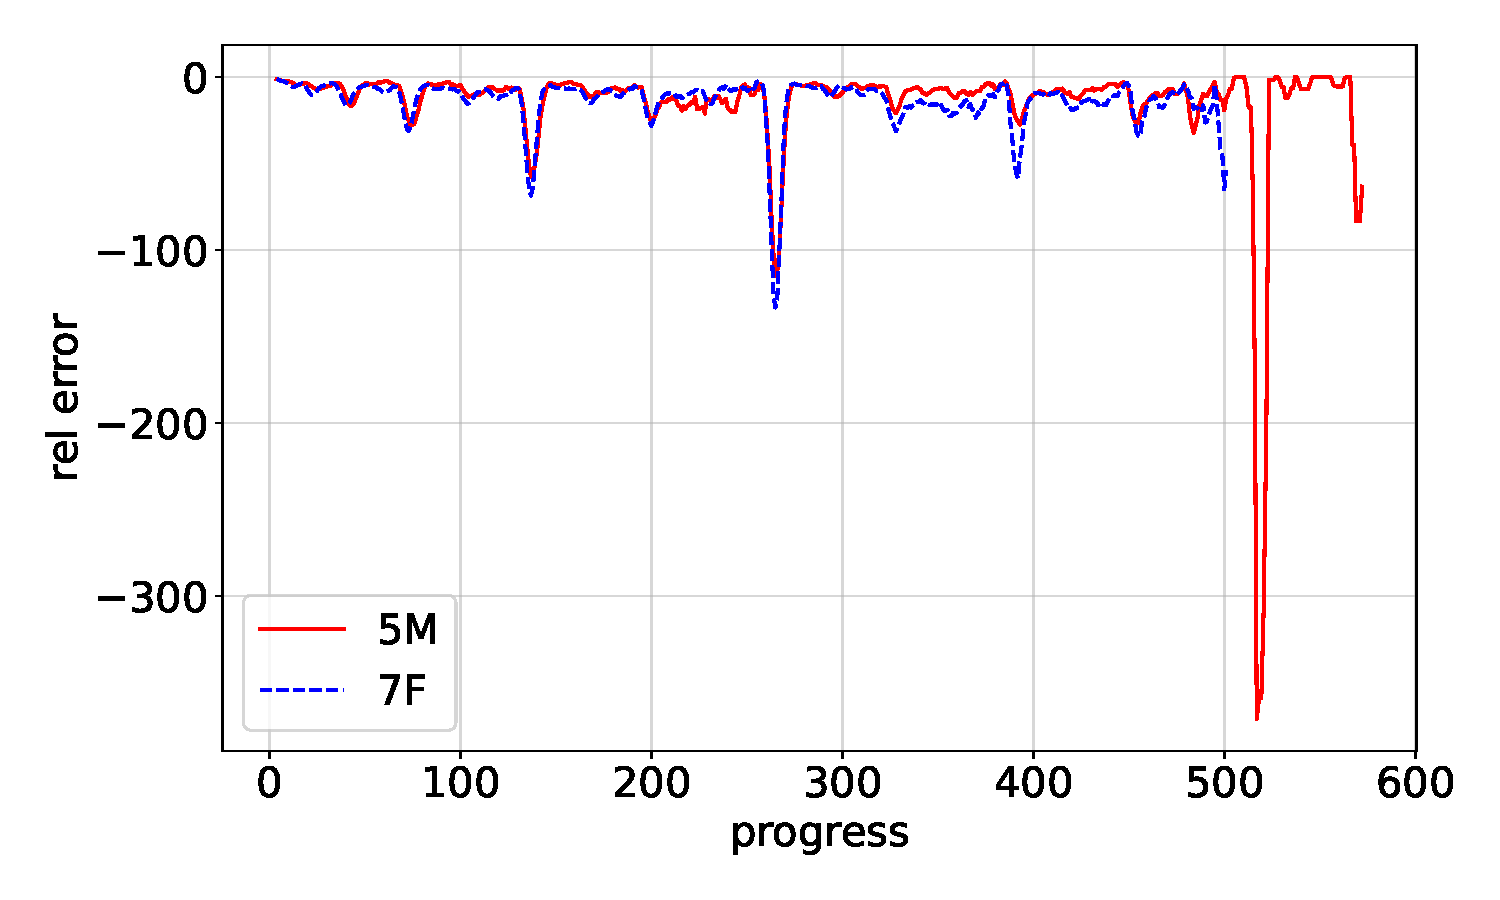
\includegraphics[width=\linewidth]{pdf/compare/NT5M_and_NT7F/error_abs.pdf}
    \caption{絶対誤差}
    \label{fig:NT5M_and_NT7F_error_abs_diff}
\end{subfigure}
\begin{subfigure}[b]{0.8\linewidth}
    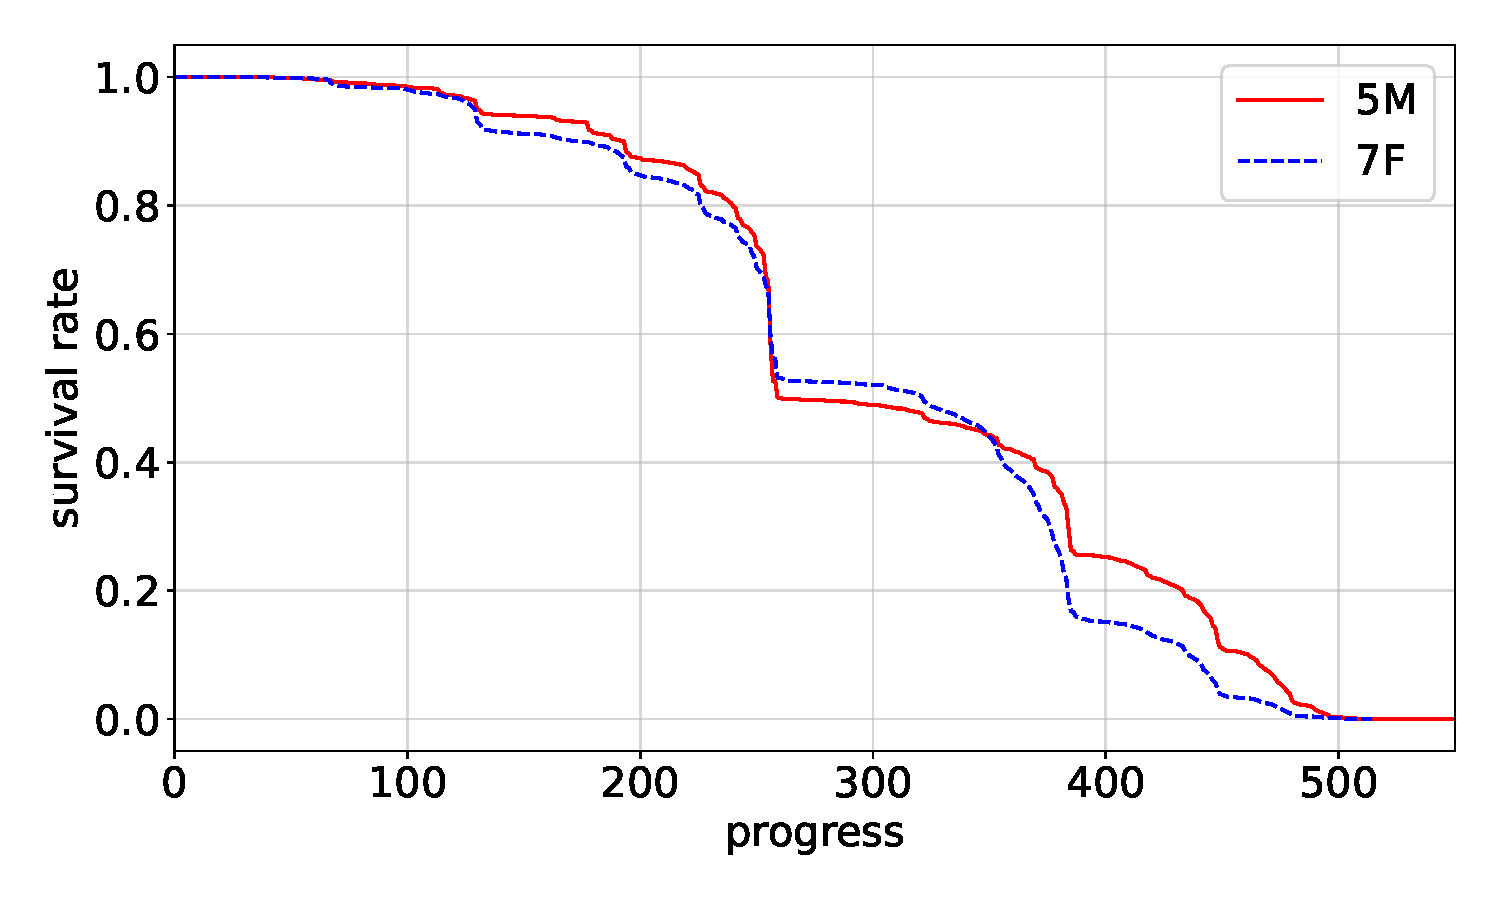
\includegraphics[width=\linewidth]{pdf/compare/NT5M_and_NT7F/survival.pdf}
    \caption{生存率}
    \label{fig:NT5M_and_NT7F_survival}
\end{subfigure}
\caption{5Mと7Fの比較結果}
\label{fig:NT5M_and_NT7F_results}
\end{figure}

次に図\ref{fig:NT5M_and_NT7F_results}は,5Mと7FのプレイヤのGreedyプレイの比較を示している.
\ref{fig:NT5M_and_NT7F_accuracy}と\ref{fig:NT5M_and_NT7F_acc_diff}を見ると
5Mの方が7Fよりも正確度が高いことが分かる.
\ref{fig:NT5M_and_NT7F_error_abs_diff}は,5Mと7Fのプレイヤの絶対誤差の差分を示している.
これを見ると,5Mの方が7Fよりも絶対誤差が小さいprogressが多いことが分かる.
\ref{fig:NT5M_and_NT7F_survival}は,5Mと7Fのプレイヤの生存率を示している.
これを見るとどちらも上下を入れ替わりながら似たような形になっていることが分かる.

図\ref{fig:NT4F_and_NT8M_results}と図\ref{fig:NT5M_and_NT7F_results}は,Greedyプレイの結果を示しているが,
どちらの結果からも特徴的な形は見られなかった.
    
\begin{figure}[t]
\centering
\begin{subfigure}[b]{0.8\linewidth}
    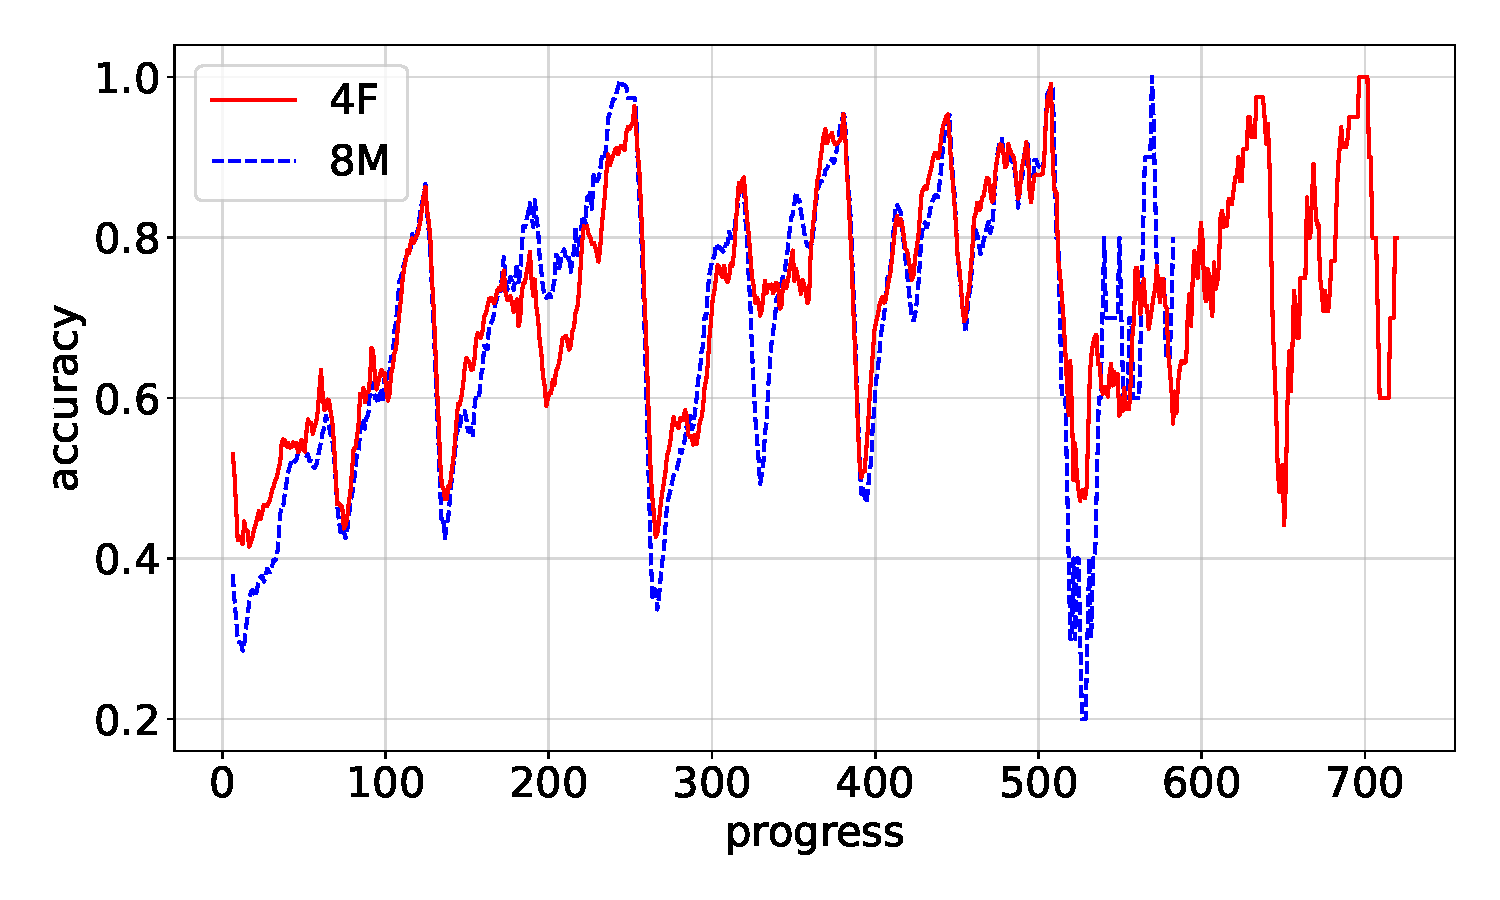
\includegraphics[width=\linewidth]{pdf/compare/EXP6_NT4F_and_NT8M/accuracy.pdf}
    \caption{正確度}
    \label{fig:EXP6_:NT4F_and_NT8M_accuracy}
\end{subfigure}
% \begin{subfigure}[b]{0.49\linewidth}
%     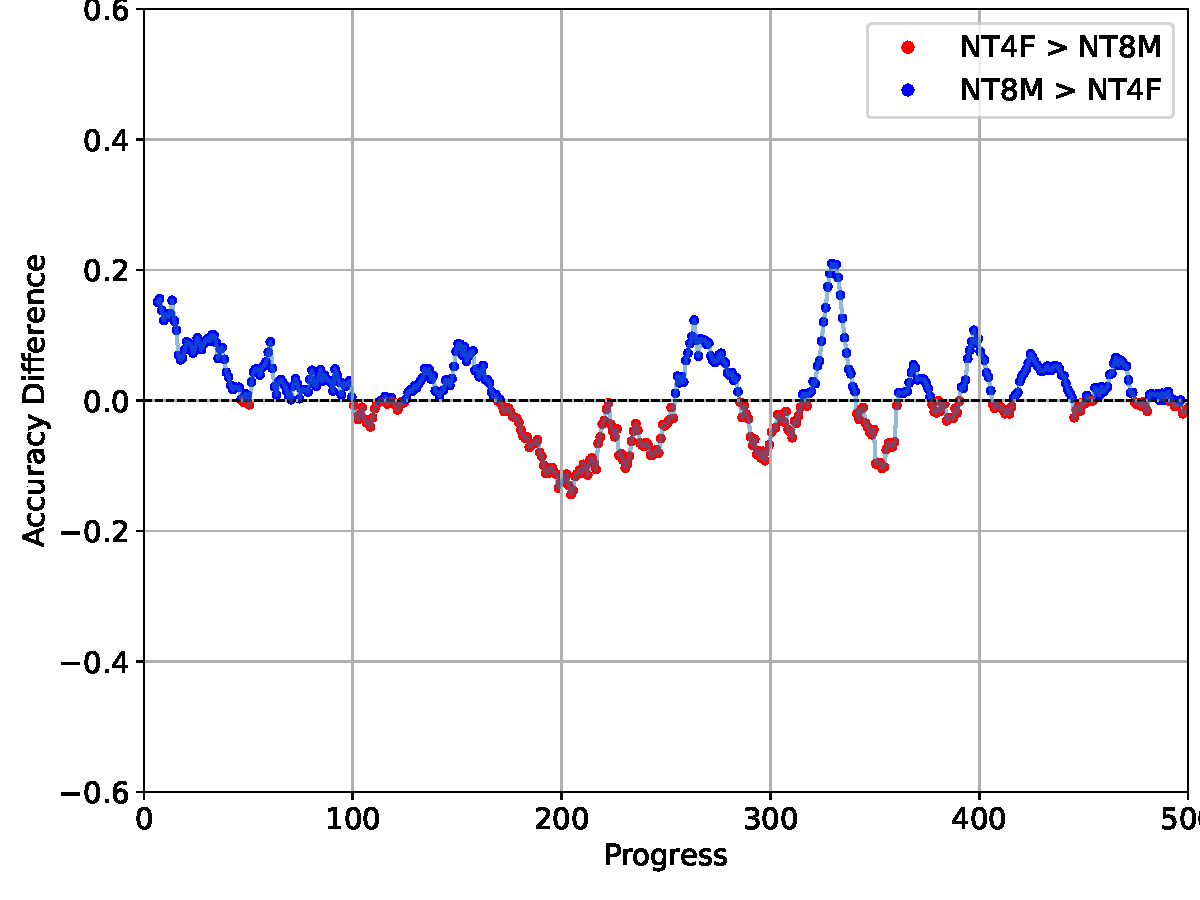
\includegraphics[width=\linewidth]{pdf/compare/EXP6_NT4F_and_NT8M/acc_diff_plot.pdf}
%     \caption{正確度の差分}
%     \label{fig:EXP6_NT4F_and_NT8M_acc_diff}
% \end{subfigure}
\begin{subfigure}[b]{0.8\linewidth}
    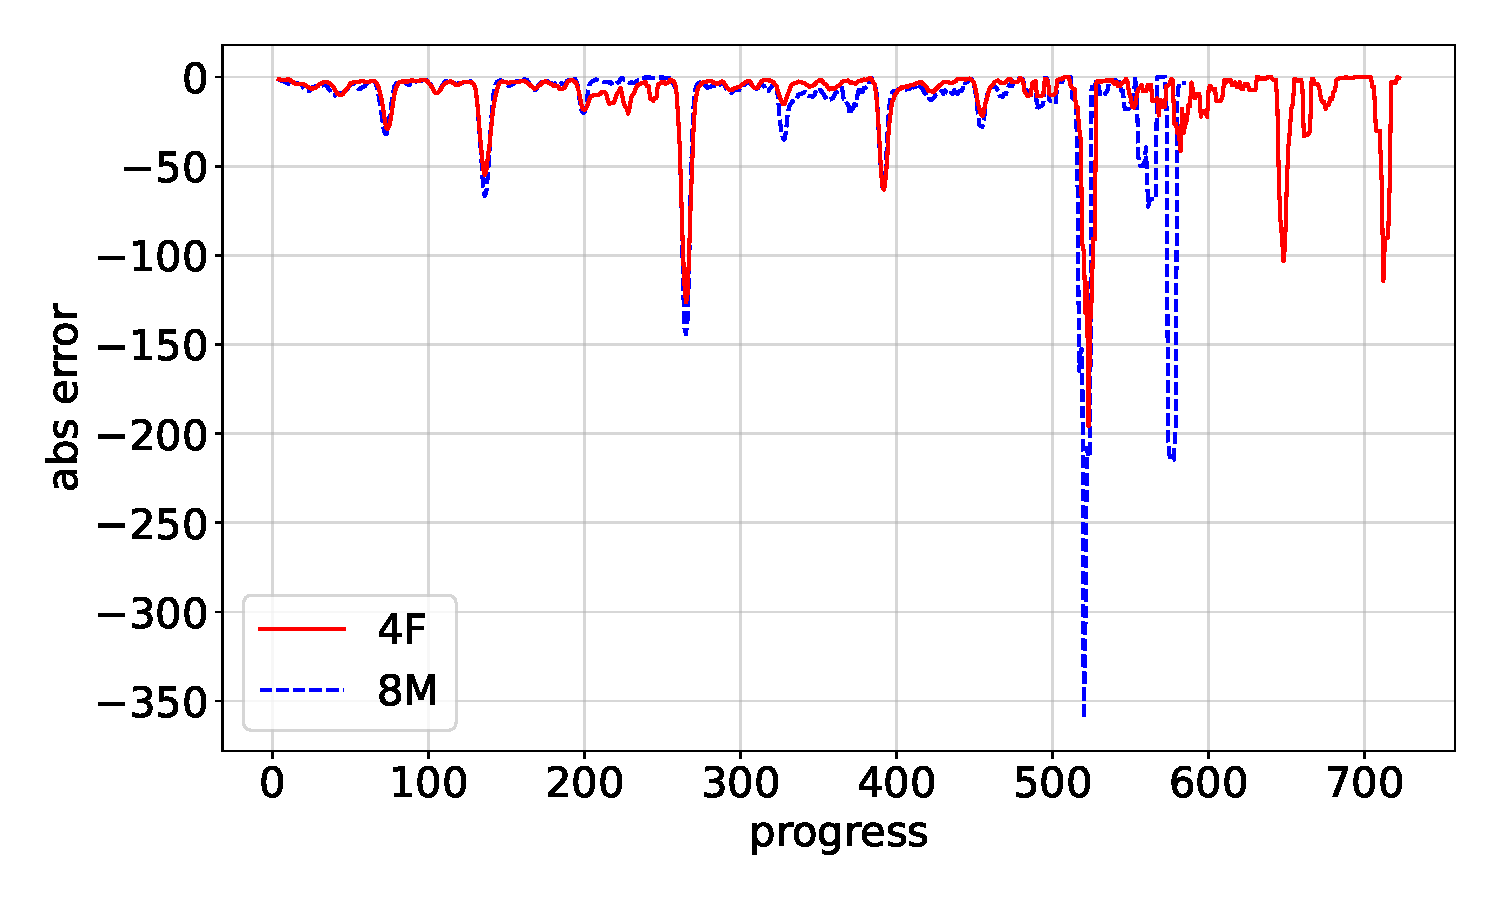
\includegraphics[width=\linewidth]{pdf/compare/EXP6_NT4F_and_NT8M/error_abs.pdf}
    \caption{絶対誤差}
    \label{fig:EXP6_NT4F_and_NT8M_error_abs_diff}
\end{subfigure}
\begin{subfigure}[b]{0.8\linewidth}
    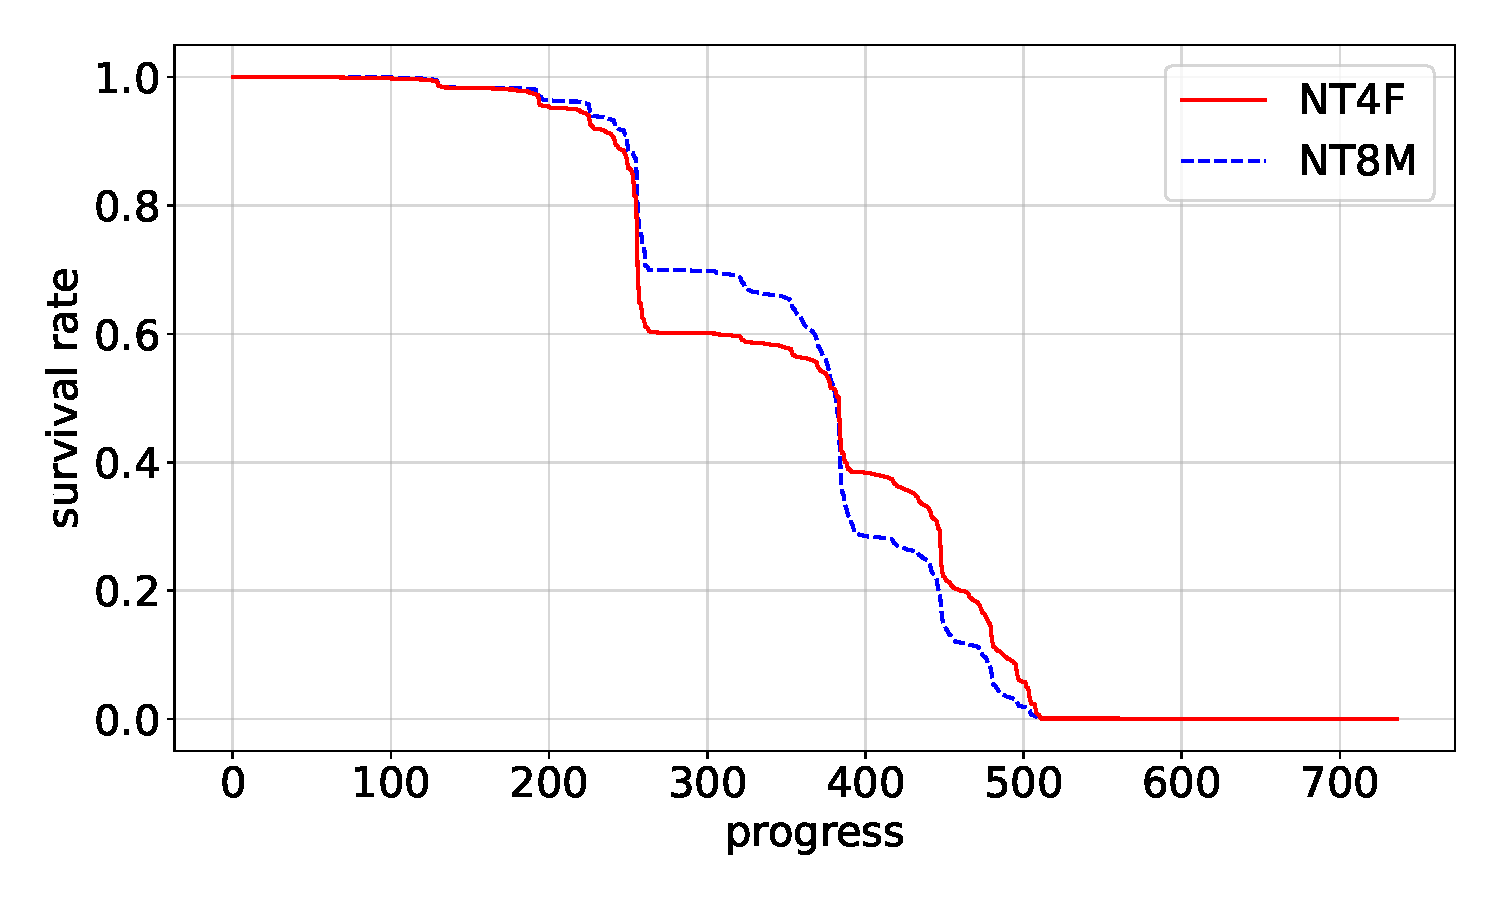
\includegraphics[width=\linewidth]{pdf/compare/EXP6_NT4F_and_NT8M/survival.pdf}
    \caption{生存率}
    \label{figEXP6_:NT4F_and_NT8M_survival}
\end{subfigure}
\caption{4Fと8Mの比較結果(深さ6)}
\label{fig:EXP6_NT4FとNT8M_results}
\end{figure}
    

\begin{figure}[t]
\centering
\begin{subfigure}[b]{0.8\linewidth}
    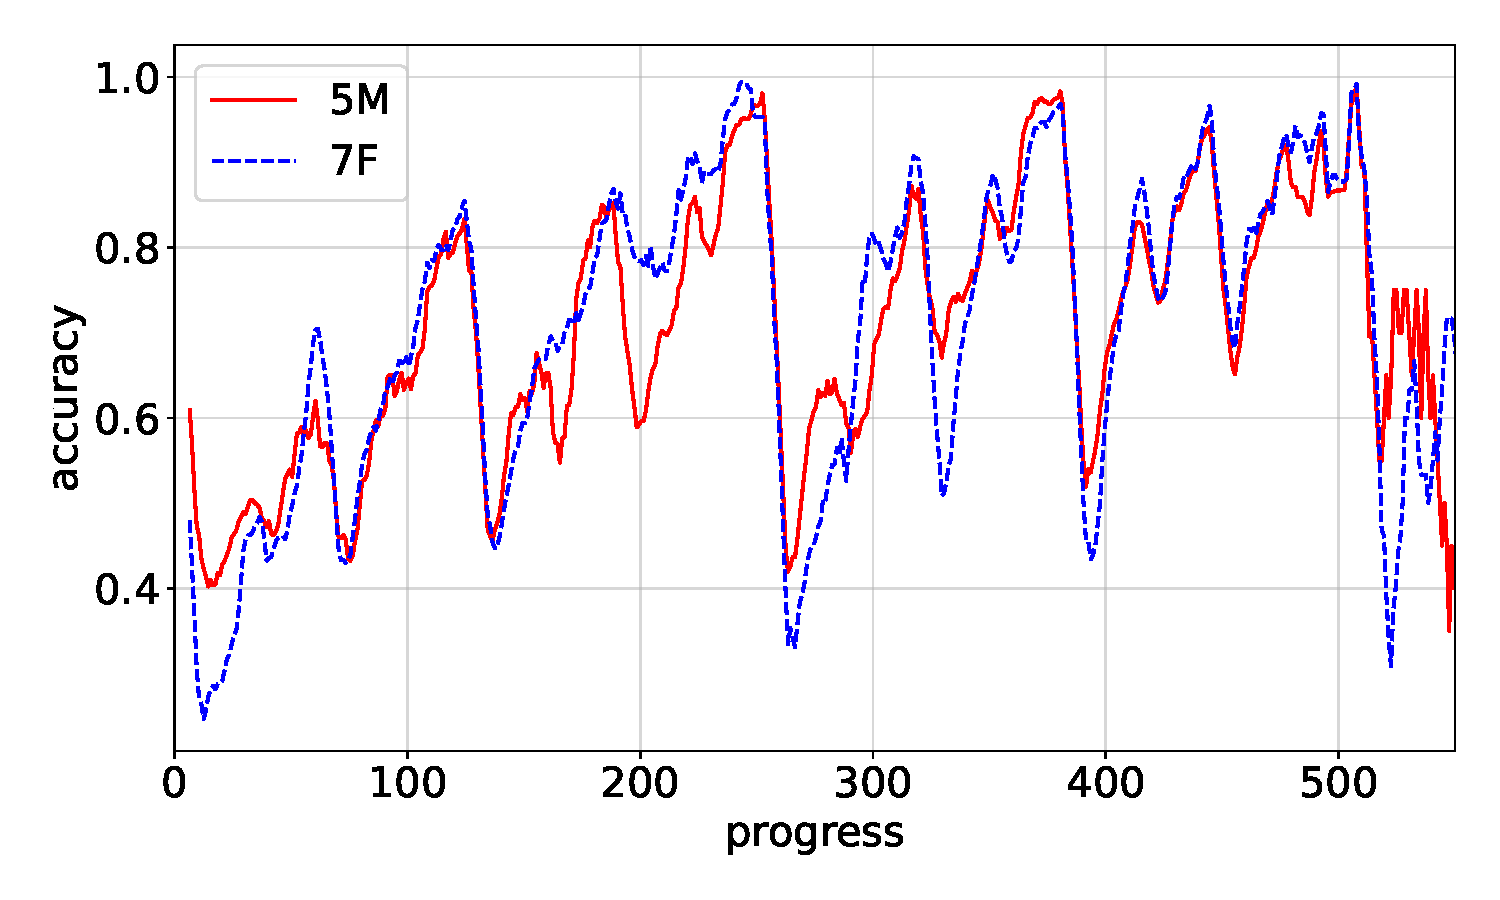
\includegraphics[width=\linewidth]{pdf/compare/EXP6_NT5M_and_NT7F/accuracy.pdf}
    \caption{正確度}
    \label{fig:EXP6_NT5M_and_NT7F_accuracy}
\end{subfigure}
% \begin{subfigure}[b]{0.8\linewidth}
%     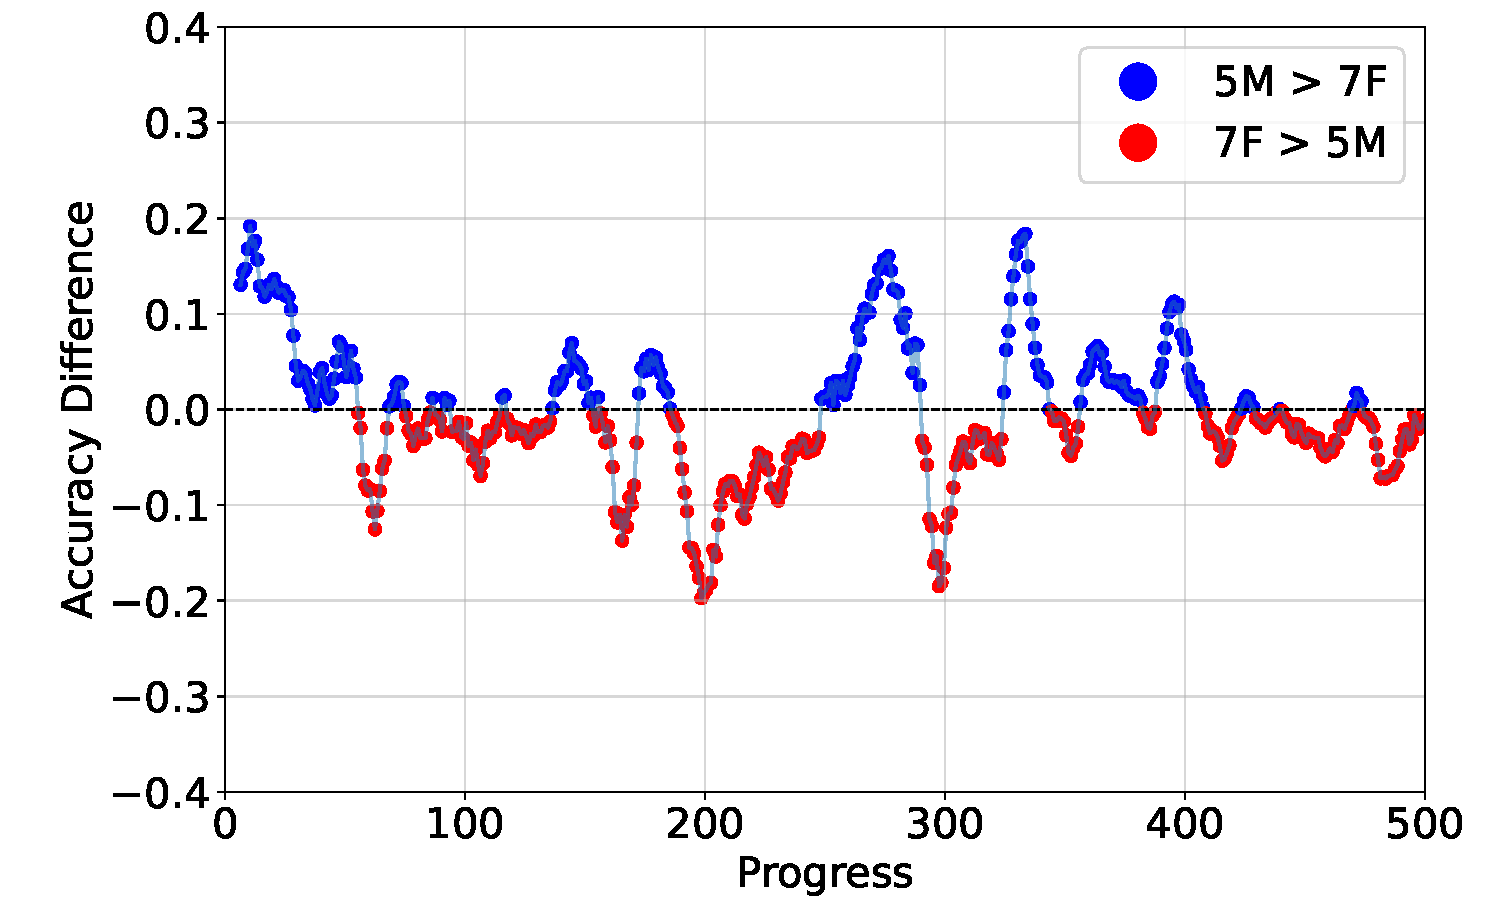
\includegraphics[width=\linewidth]{pdf/compare/EXP6_NT5M_and_NT7F/acc_diff_plot.pdf}
%     \caption{正確度の差分}
%     \label{fig:EXP6_NT5M_and_NT7F_acc_diff}
% \end{subfigure}
\begin{subfigure}[b]{0.8\linewidth}
    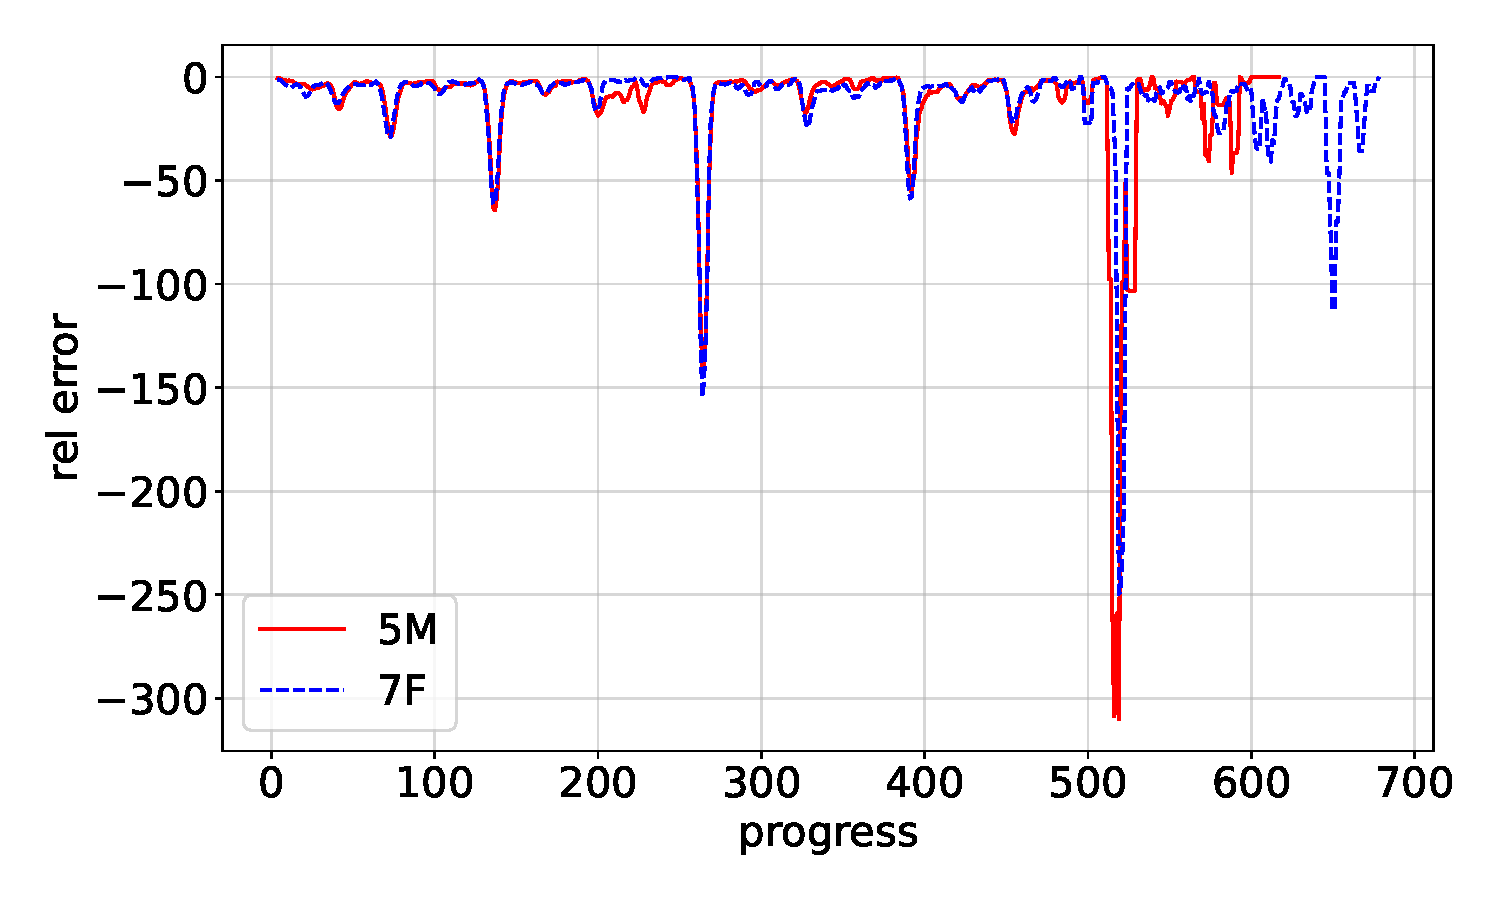
\includegraphics[width=\linewidth]{pdf/compare/EXP6_NT5M_and_NT7F/error_abs.pdf}
    \caption{絶対誤差}
    \label{fig:EXP6_NT5M_and_NT7F_error_abs_diff}
\end{subfigure}
\begin{subfigure}[b]{0.8\linewidth}
    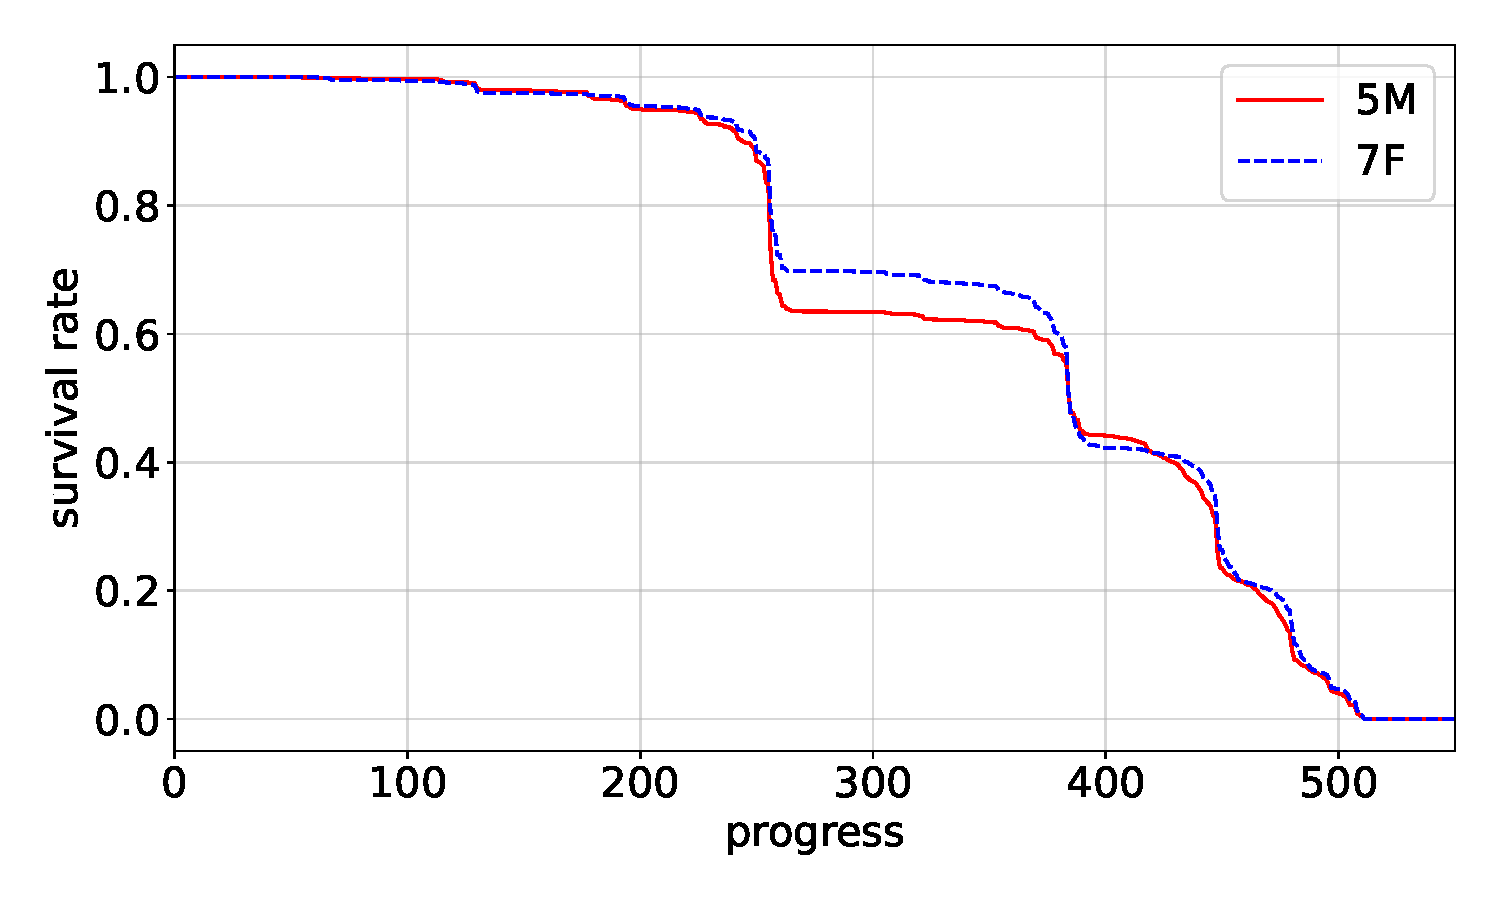
\includegraphics[width=\linewidth]{pdf/compare/EXP6_NT5M_and_NT7F/survival.pdf}
    \caption{生存率}
    \label{fig:EXP6_NT5M_and_NT7F_survival}
\end{subfigure}
\caption{5Mと7Fの比較結果(深さ6)}
\label{fig:EXP6_NT5M_and_NT7F_results}
\end{figure}

図\ref{fig:EXP6_NT4FとNT8M_results}と図\ref{fig:EXP6_NT5M_and_NT7F_results}は,
図\ref{fig:NT4F_and_NT8M_results}と図\ref{fig:NT5M_and_NT7F_results}のExpectimax探索深さ6を組み合わせたプレイヤである.
図\ref{fig:EXP6_:NT4F_and_NT8M_accuracy}と図\ref{fig:EXP6_NT4F_and_NT8M_acc_diff}を見ると正確性はNT4Fの方が良い
図\ref{fig:EXP6_NT5M_and_NT7F_accuracy}と図\ref{fig:EXP6_NT5M_and_NT7F_acc_diff}を見ると正確性はNT5Mの方が良い
図\ref{fig:EXP6_NT4F_and_NT8M_error_abs_diff}と図\ref{fig:EXP6_NT5M_and_NT7F_error_abs_diff}は絶対誤差の差分を示していて,
ここは探索を加えたことで上下の振れ幅がとても小さくなっていることが分かるが結局どちらの結果からも特徴的な形は見られなかった.
